\documentclass[10.5pt]{config}
% 本实验报告采用 署名-相同方式共享 4.0 国际许可协议 (CC BY-SA 4.0)
\usepackage{bigstrut,multirow,rotating,booktabs,makecell,array}%表格插件
\usepackage{color, xcolor}

\major{电子科学与技术}
\name{郑智瑄，徐棵}
\partner{} % 签名栏
% \title{}
\stuid{3230103913，3230104003}
\date{\today}
\lab{东4-421}
\course{电子工程训练（甲）}
\instructor{李培弘}
\grades{}
\expname{电子工训智能插座DIY项目} % 实验名字
\exptype{测试型} % 实验类型

\begin{document}

% \maketitlepage % 封面
% \maketoc % 目录
\makeheader % 首页头部

\section{电装}
\subsection{电装元器件顺序}
为方便焊接，我们采取了先低后高的焊接顺序，
首先焊接了最低的电阻与二极管1N4148，
然后焊接较低的瓷片电容、继电器插座/芯片插座、
Type-C USB插口、发光二极管与三极管，
接着焊接了较高的按钮、电解电容、温度传感器插座、可变电阻、正面排针，
最后焊接了最高的双联USB接口和自锁开关
\subsection{供电电路测试}
\begin{enumerate}
  \item Type-C插上外接5V电源，观察“D3”是否亮起
  \item 用万用表的直流电压档，检查J1排针上的第3脚（标注5V）与4或5脚（标注GND）之间的5V电压是否正确
  \item 用万用表的直流电压档测量USB电压是否与外接5V电源电压一致，即约5V。电压表的负极表棒接电路系统的地线端GND（TP3）
\end{enumerate}
\begin{figure}[H]
  \centering
  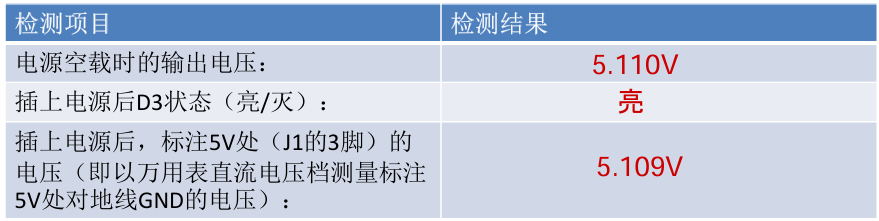
\includegraphics[width=0.7\linewidth]{figures/f11.png} % 数字表示放缩比例
  \caption{供电电路测试结果} % 图片标题
\end{figure}
【结果分析】：供电电路无问题，能正常运行

\subsection{USB插座供电控制电路}
\subsubsection{USB2信号路径分析}
\begin{figure}[H]
  \centering
  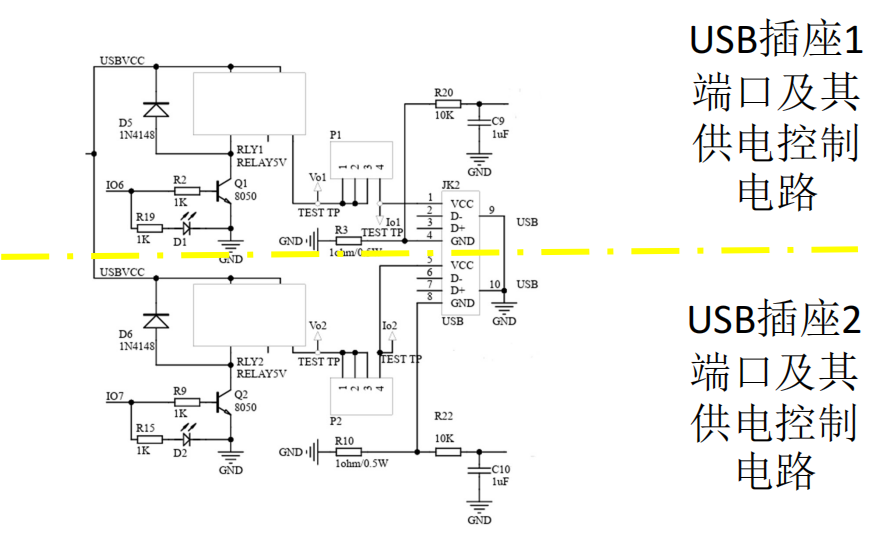
\includegraphics[width=0.5\linewidth]{figures/p11.png} % 数字表示放缩比例
  \caption{USB插座供电控制电路} % 图片标题
\end{figure}
【USB2信号路径分析】：引脚IO7通过高/低电平（即+5V/0V），可控制三极管Q2的导
通/截止，从而决定继电器RLY2的通断，最终决定USB供
电插座JK2上的USB2口是否有5V（即USBVCC）电源输出。
供电电流将从USB2口的VCC引脚流出，经过外接用电器，
从USB2口的GND流回。
\subsubsection{USB插座供电控制电路测试}
\begin{enumerate}
  \item 测试插座供电输出控制功能是否完备：首先连接一根杜邦线到J1排针的第3脚（即5V）
  \item 测试USB供电插座JK2的USB1口的输出控制：将杜邦线另一端连接到排针J3的第7脚（即L1）
  \item 测试USB供电插座JK2的USB2口的输出控制：将原先连接J3排针第7脚的杜邦线一端连接到J3排针的第8脚（即L2）
  \begin{figure}[H]
    \centering
    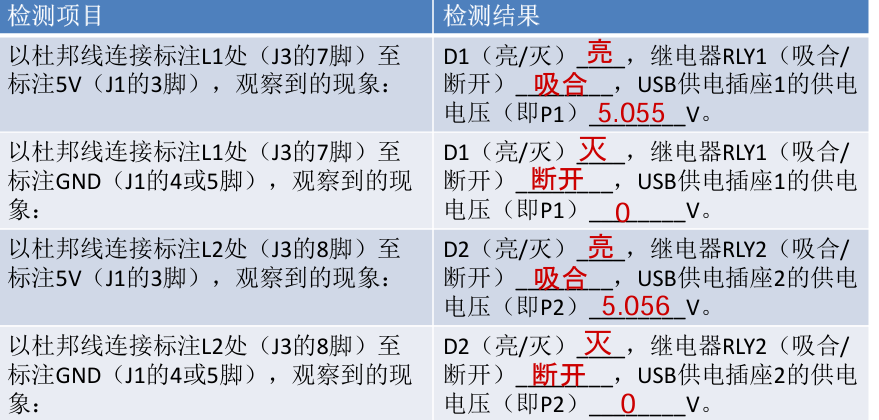
\includegraphics[width=0.7\linewidth]{figures/f12.png} % 数字表示放缩比例
    \caption{USB插座供电控制电路测试结果} % 图片标题
  \end{figure}
\end{enumerate}
【结果分析】：USB插座供电控制电路无问题，能正常运行
\subsection{指示灯与按钮电路测试}
\begin{figure}[H]
  \centering
  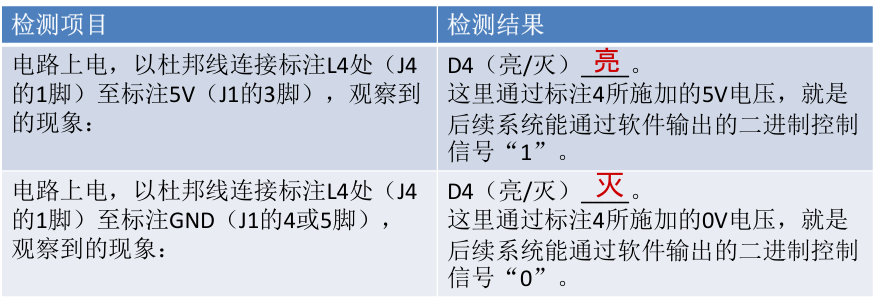
\includegraphics[width=0.7\linewidth]{figures/f13.png} % 数字表示放缩比例
  \caption{指示灯测试结果} % 图片标题
\end{figure}
【结果分析】：指示灯控制电路无问题，能正常运行
\subsection{电装总体完成后的初步通电测试}
\begin{enumerate}
  \item 先不安装芯片LM324AN和LM35DZ，通过接入外接5V直流稳压电源，进行初步的通电测试。
  \item 检查U1（即LM324AN）芯片插座上的电源电压（即该插座上4脚和11脚之间的电压）是否为正常的5V，并记录检测结果。
  \item 检查U2（即LM35DZ）芯片插座上的电源电压是否为正常的5V（即该插座上1脚和3脚之间的电压），并记录检测结果。断开外接5V直流稳压电源。
  \item 上述电压均检测无误后，将芯片LM324AN和芯片LM35DZ安插到其相应的插座上。
  \begin{figure}[H]
    \centering
    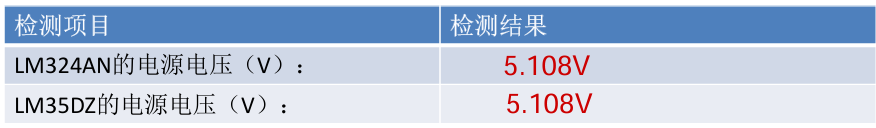
\includegraphics[width=0.7\linewidth]{figures/f14.png} % 数字表示放缩比例
    \caption{集成电路芯片的供电检测结果} % 图片标题
  \end{figure}
\end{enumerate}
【结果分析】：集成电路芯片的供电无问题，能正常运行
\section{调试}
\subsection{基于硬件调整的温度值标定调试}
【实验步骤】：电路中的可变电阻VR1用于调整温度测量值输入时的转换比例，所以需要根据在测试程序中显示的温度值，同时参考当前室温（通过我
们教室中安放的温度计来读取），并通过调整可变电阻VR1
的螺丝旋钮来调整显示值，并使之与实际室温的尽量保持一致
\begin{figure}[H]
  \centering
  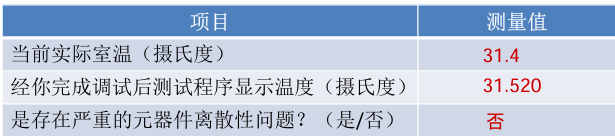
\includegraphics[width=0.7\linewidth]{figures/f21.png} % 数字表示放缩比例
  \caption{供电电路测试结果} % 图片标题
\end{figure}
【结果分析】：无明显元器件离散问题，可与实际室温拟合

\subsection{基于软件后处理的电流数据标定}
\subsubsection{采样电流数据}
\begin{figure}[H]
  \centering
  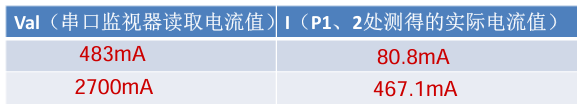
\includegraphics[width=0.7\linewidth]{figures/f22.png} % 数字表示放缩比例
  \caption{供电电路测试结果} % 图片标题
\end{figure}
\subsubsection{标定公式}
计算求解k,b,最终的标定公式为：
$$I = 0.174Val – 3.242$$
\begin{figure}[H]
  \centering
  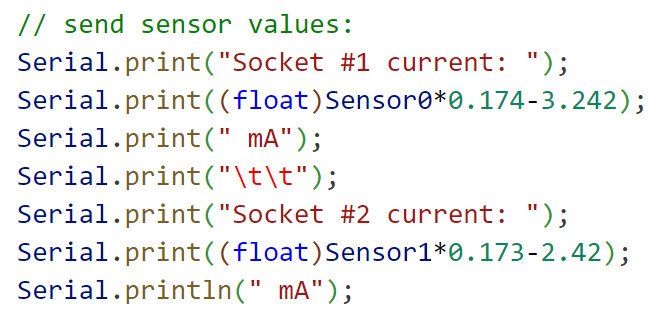
\includegraphics[width=0.7\linewidth]{figures/I.jpg} % 数字表示放缩比例
  \caption{修改后代码段} % 图片标题
\end{figure}
\subsubsection{数据采集与误差分析}
用你标定好的小程序，采集量程范围内的10个值，并比较其与电流表实际读数的差异
\begin{table}[H]
  \centering
    \begin{tabular}{|c|c|c|}
    \hline
    \multicolumn{1}{|p{15.065em}|}{Val（串口监视器读取电流值）/mA} & \multicolumn{1}{p{15em}|}{I（P1、2处测得的实际电流值）/mA} & \multicolumn{1}{p{2.235em}|}{误差} \bigstrut\\
    \hline
    80.63 & 80.8  & 0.21\% \bigstrut\\
    \hline
    118.56 & 118.8 & 0.20\% \bigstrut\\
    \hline
    162.06 & 162.5 & 0.27\% \bigstrut\\
    \hline
    213.56 & 214   & 0.21\% \bigstrut\\
    \hline
    238.27 & 237.8 & 0.20\% \bigstrut\\
    \hline
    260.89 & 260.6 & 0.11\% \bigstrut\\
    \hline
    278.29 & 277.5 & 0.28\% \bigstrut\\
    \hline
    322.49 & 321.2 & 0.40\% \bigstrut\\
    \hline
    353.98 & 353.7 & 0.08\% \bigstrut\\
    \hline
    410.18 & 411.4 & 0.30\% \bigstrut\\
    \hline
    467.25 & 467.5 & 0.05\% \bigstrut\\
    \hline
    \end{tabular}%
  \caption{CH1 数据采集与误差分析}
  \label{tab:addlabel}%
\end{table}%
\subsubsection{另一路电流标定}
同上进行电流标定，结果如下：

$$I = 0.173Val – 2.24$$
% Table generated by Excel2LaTeX from sheet 'Sheet1'
% Table generated by Excel2LaTeX from sheet 'Sheet1'
\begin{table}[H]
  \centering
    \begin{tabular}{|c|c|c|}
    \hline
    \multicolumn{1}{|p{15.065em}|}{Val（串口监视器读取电流值）/mA} & \multicolumn{1}{p{15em}|}{I（P1、2处测得的实际电流值）/mA} & \multicolumn{1}{p{2.235em}|}{误差} \bigstrut\\
    \hline
    80.62 & 80.8  & 0.22\% \bigstrut\\
    \hline
    105.53 & 105.9 & 0.35\% \bigstrut\\
    \hline
    217.29 & 217.9 & 0.28\% \bigstrut\\
    \hline
    249.47 & 249.2 & 0.11\% \bigstrut\\
    \hline
    274.03 & 273.9 & 0.05\% \bigstrut\\
    \hline
    303.44 & 303.1 & 0.11\% \bigstrut\\
    \hline
    334.76 & 334.8 & 0.01\% \bigstrut\\
    \hline
    378.7 & 378.7 & 0.00\% \bigstrut\\
    \hline
    406.03 & 407   & 0.24\% \bigstrut\\
    \hline
    426.1 & 427.7 & 0.37\% \bigstrut\\
    \hline
    469.87 & 470.4 & 0.11\% \bigstrut\\
    \hline
    \end{tabular}%
  \label{tab:addlabel}%
  \caption{CH2 数据采集与误差分析}
\end{table}%
【结果分析】：经标定后，串口监视器读得两路电流与实际电流值拟合较好，误差较小

\subsection{软硬件相结合的系统调试}
\subsubsection{测试任务一}
【实验步骤】：利用小台灯和小程序$SmtScktTest\_USB$，确认程序控制USB插座中1\#和2\#的插座分别由哪个引脚控制
\begin{figure}[H]
  \centering
  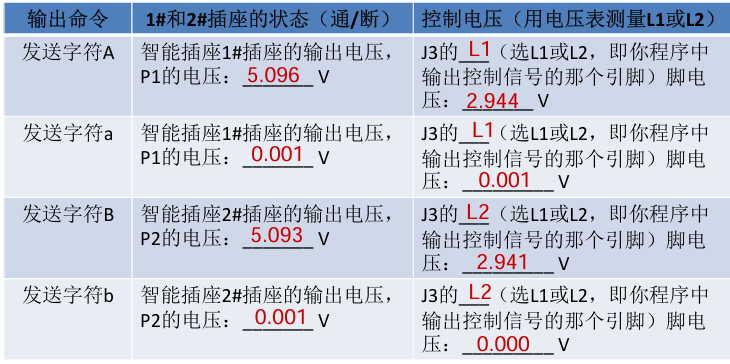
\includegraphics[width=0.7\linewidth]{figures/f24.png} % 数字表示放缩比例
  \caption{测试任务一测试结果}
\end{figure}

【结果分析】：1\#插座由“A"和“a”控制开关，2\#插座由“B"和“b”控制开关
\subsubsection{测试任务二}
【实验步骤】：利用各类用电器，测量其在智能插座使用中的各类测量值
\begin{figure}[H]
  \centering
  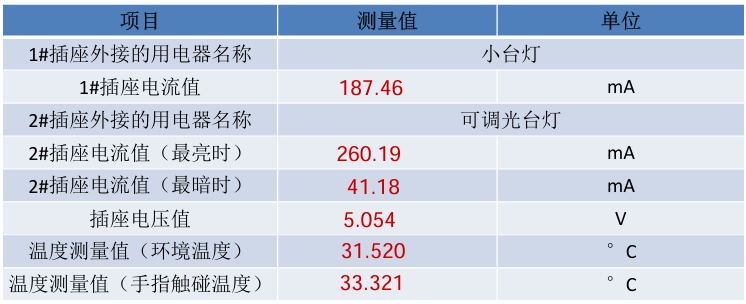
\includegraphics[width=0.7\linewidth]{figures/f25.png} % 数字表示放缩比例
  \caption{测试任务二测试结果}
\end{figure}
\subsubsection{测试任务三}
【实验步骤】：将2\#插座上的可调光台灯换成风扇，并接通风扇的插座电源，测量风扇的各档工作电流值。
\begin{figure}[H]
  \centering
  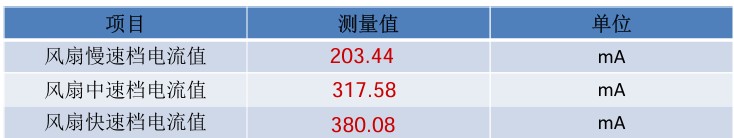
\includegraphics[width=0.7\linewidth]{figures/f26.png} % 数字表示放缩比例
  \caption{测试任务三测试结果}
\end{figure}
【实验异常分析】：
上述测试任务（2）、（3）中有哪些测量值有异常？利用示波器观察并拍照记录出现这些异常时输出供电电压的波形，说明其产生的原因。
\begin{figure}[H]
  \centering
  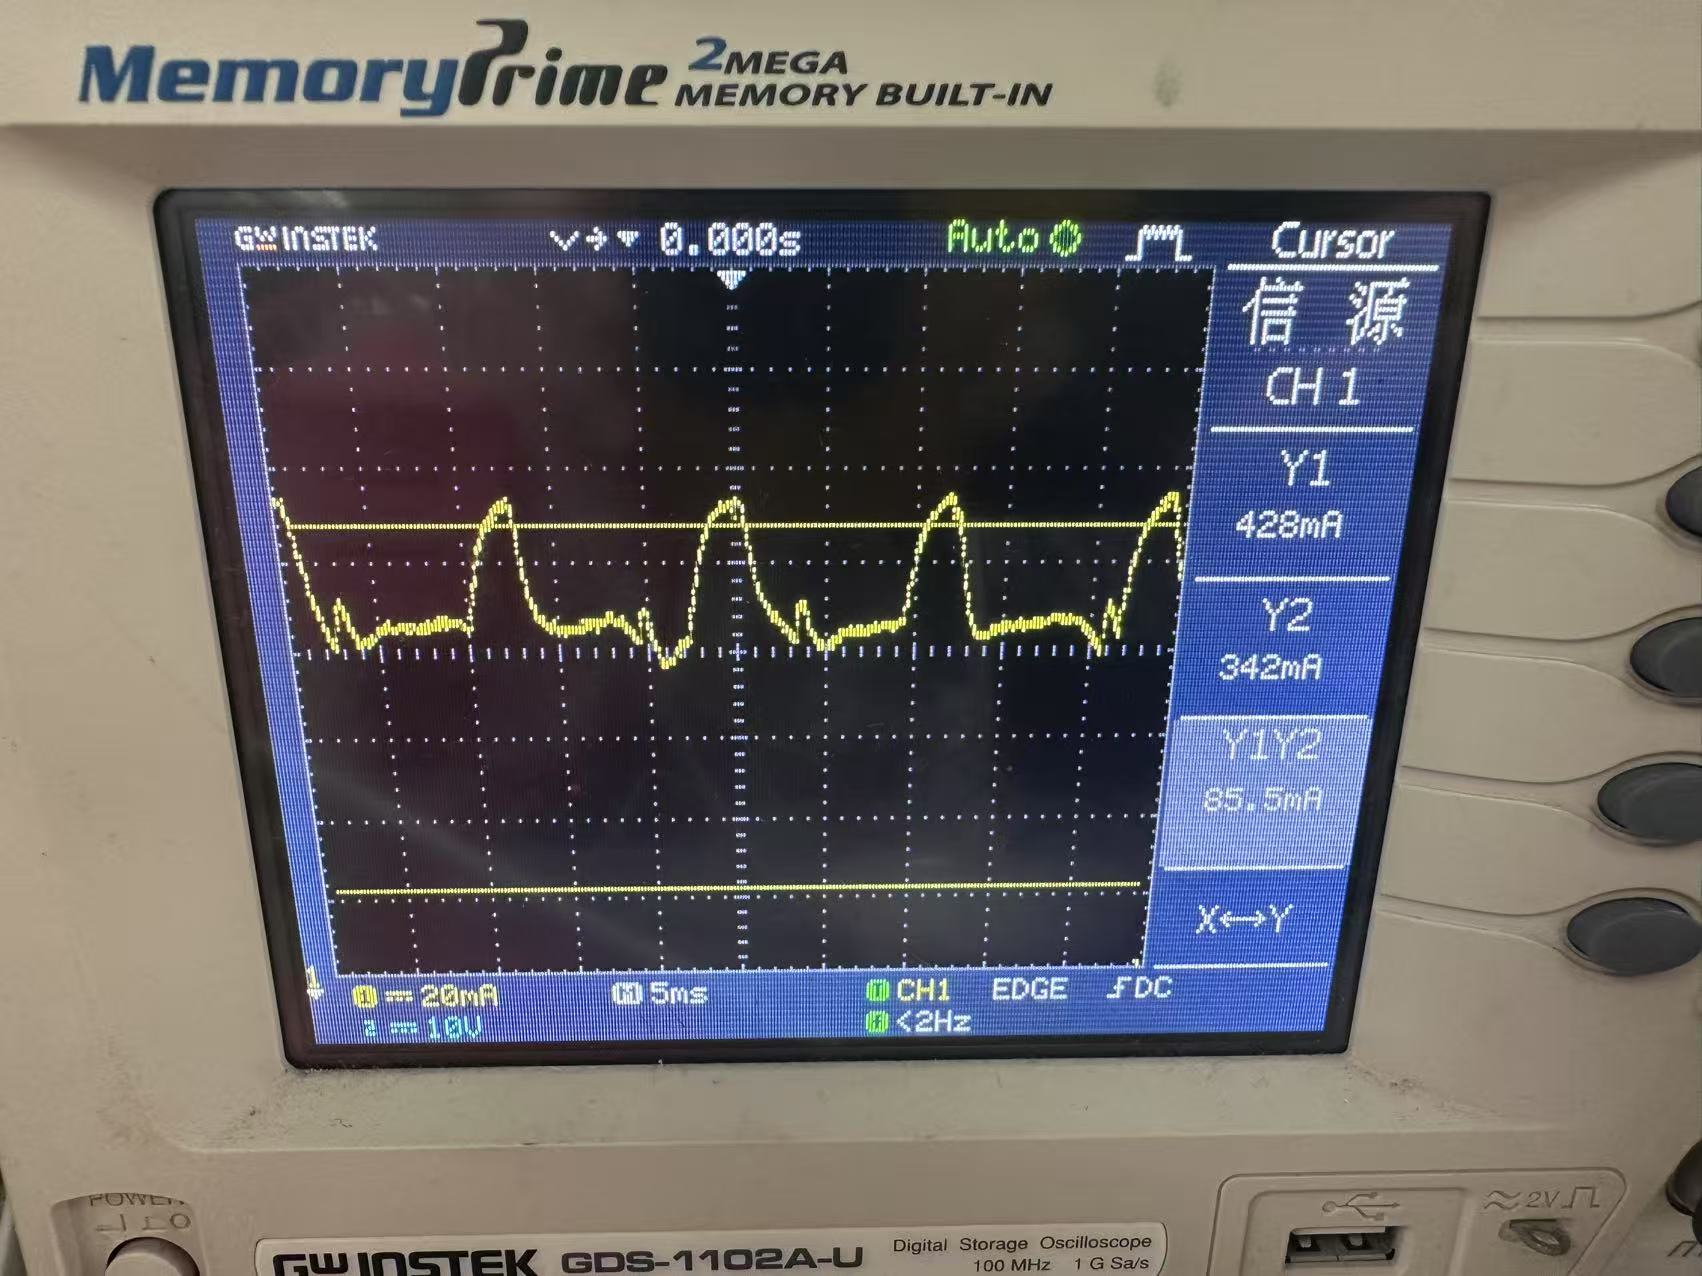
\includegraphics[width=0.5\linewidth]{figures/t3.jpg} % 数字表示放缩比例
  \caption{异常输出供电电压波形}
\end{figure}
【异常值】：任务三中测量风扇的各档工作电流值时电流值约有$\pm$ 20mA的波动

【分析】：小风扇由PWM驱动，PWM为脉冲电压信号，电流会随着脉冲的高低电平变化而周期性变动

\subsection{软硬件联调任务一}
【实验要求】：
在我们的智能插座给风扇供电时，会出现电流值不停地大小
波动变化的现象，这是由于该风扇的调速采用了
方式PWM的控制请在
$SmtScktTest\_USB.ino$
程序中添加一个子程序，通过调用
该子程序，实现对采集的电流值取平均值，以便使同一转速
挡位的电流值显示趋于平稳。

【提示】：
在取平均值时，可以选择给以往值和当前值取不同的权值，
即\colorbox{yellow}{加权平均法}；也可以选择\colorbox{yellow}{移动平均法}等，来调整平均值的
计算效果，以达到既能在风扇档位变化时，尽快地响应电流
的变化，同时又能在各档位保持不变时，使电流的显示值趋
于平稳。

【代码与实现方式】：我们选择了\colorbox{yellow}{移动平均法}来使电流显示值平稳，$movingAverageFilter$函数
可对输入的电流值用移动平均法进行滤波，其操作过程如下：

在读取原始电流值后，通过参数传递原始值、样本数组、索引和累加和，在函数中，通过滑动窗口动态更新平均值，采用环形缓冲区索引管理
来移除最旧值，添加最新值，最后返回窗口内数组的平均值

本次实验中，通过定义宏窗口大小WINDOW\_SIZE来平衡尽快响应电流变化，
与电流的显示值平稳的要求，当提高WINDOW\_SIZE时，电流的显示值趋于平稳，但响应变慢，
当减小WINDOW\_SIZE时，响应变快，但显示值波动较大，经过实验测试，最终发现当WINDOW\_SIZE为8时，
电流显示值较为平稳且响应较快，故最终取WINDOW\_SIZE为8
\begin{figure}[H]
  \centering
  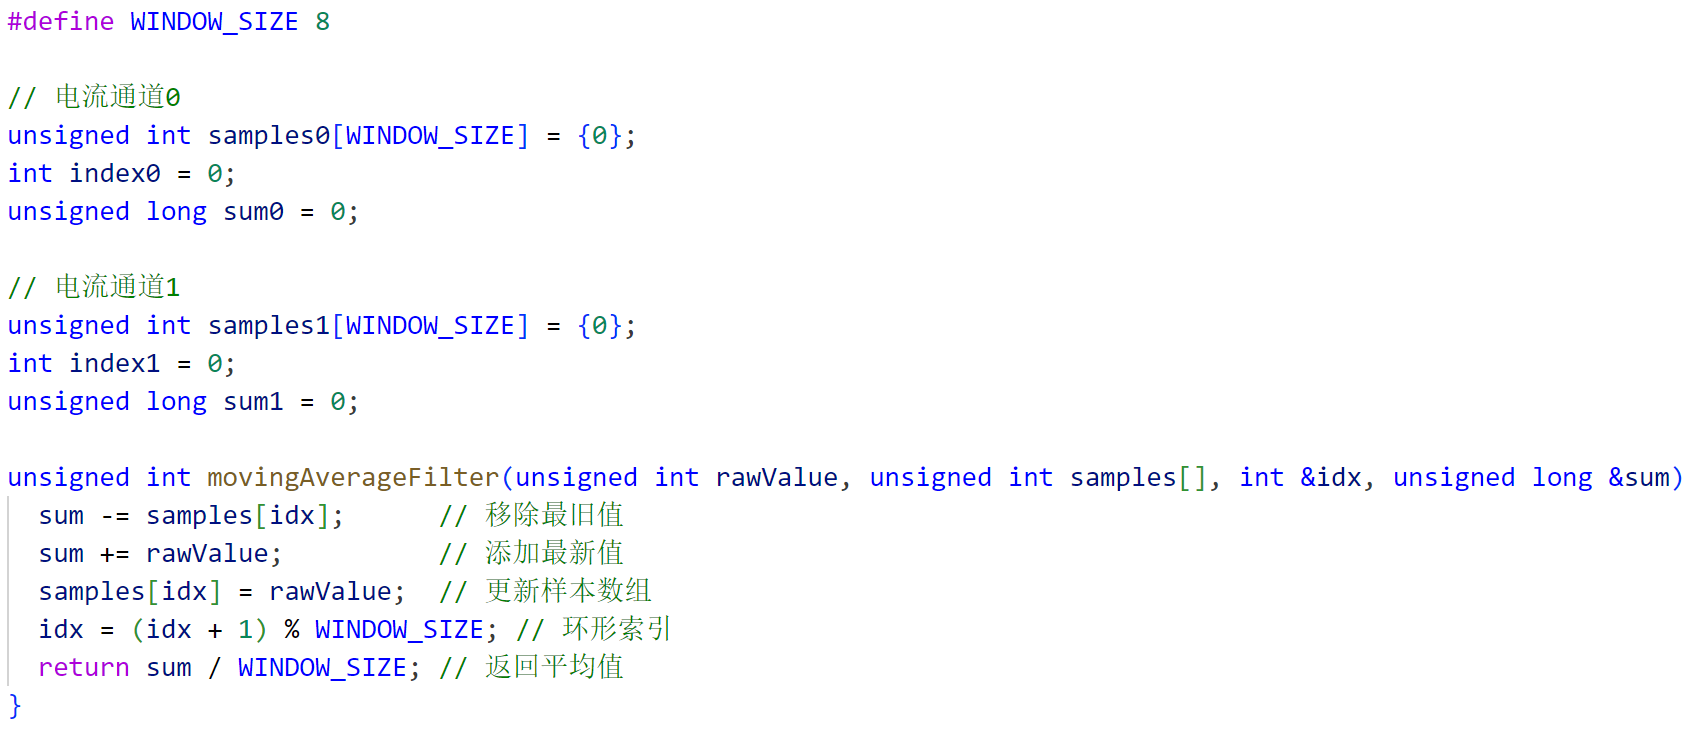
\includegraphics[width=1\linewidth]{figures/pwm1.png} % 数字表示放缩比例
  \caption{软硬件联调任务一代码段}
\end{figure}

\begin{figure}[H]
  \centering
  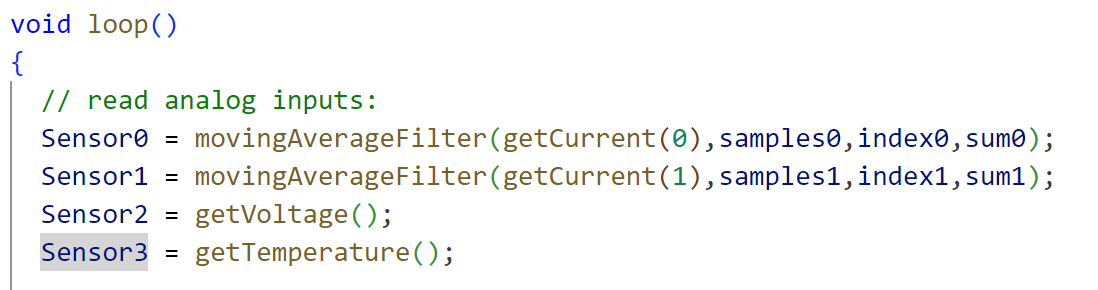
\includegraphics[width=1\linewidth]{figures/pwm2.png} % 数字表示放缩比例
  \caption{软硬件联调任务一代码段}
\end{figure}


\subsection{软硬件联调任务四}
\subsubsection{步骤1}

【实验要求】：
首先弄清按下按钮/
松开按钮时，
Arduino程序分别读取到的按键状态值（二进制的
0/1）。
在按钮保持在按下或松开时，按下‘k’命令，以便确定按钮被按下时，被
读取到的按钮状态值值是
Arduino程序0还是
1？

\begin{figure}[H]
  \centering
  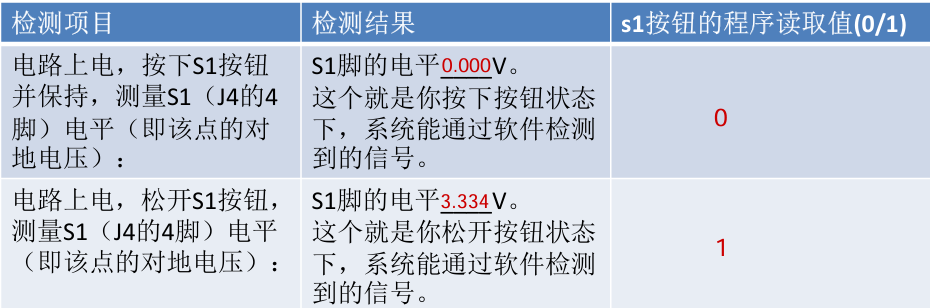
\includegraphics[width=0.7\linewidth]{figures/f27.png} % 数字表示放缩比例
  \caption{软硬件联调任务四表}
\end{figure}

\subsubsection{步骤2}

【实验要求】：
采用各种按键速度和连续按键次数，
测试程序是否能每次都正确记录按钮次数？如果不是
（即存在误读次数）
通过示波器查看并记录按钮
按动时的波形，并分析误读产生的原因

【示波器显示结果】：
改变按键速度与连续按键次数，可能由于此按钮机械性能较好，各种情况下毛刺数量并没有很多，一般均得到左图类似图片，多次尝试才
得到如下右图毛刺图片
\begin{figure}[H]
  \centering
  \begin{minipage}[b]{0.5\linewidth}
      \centering
      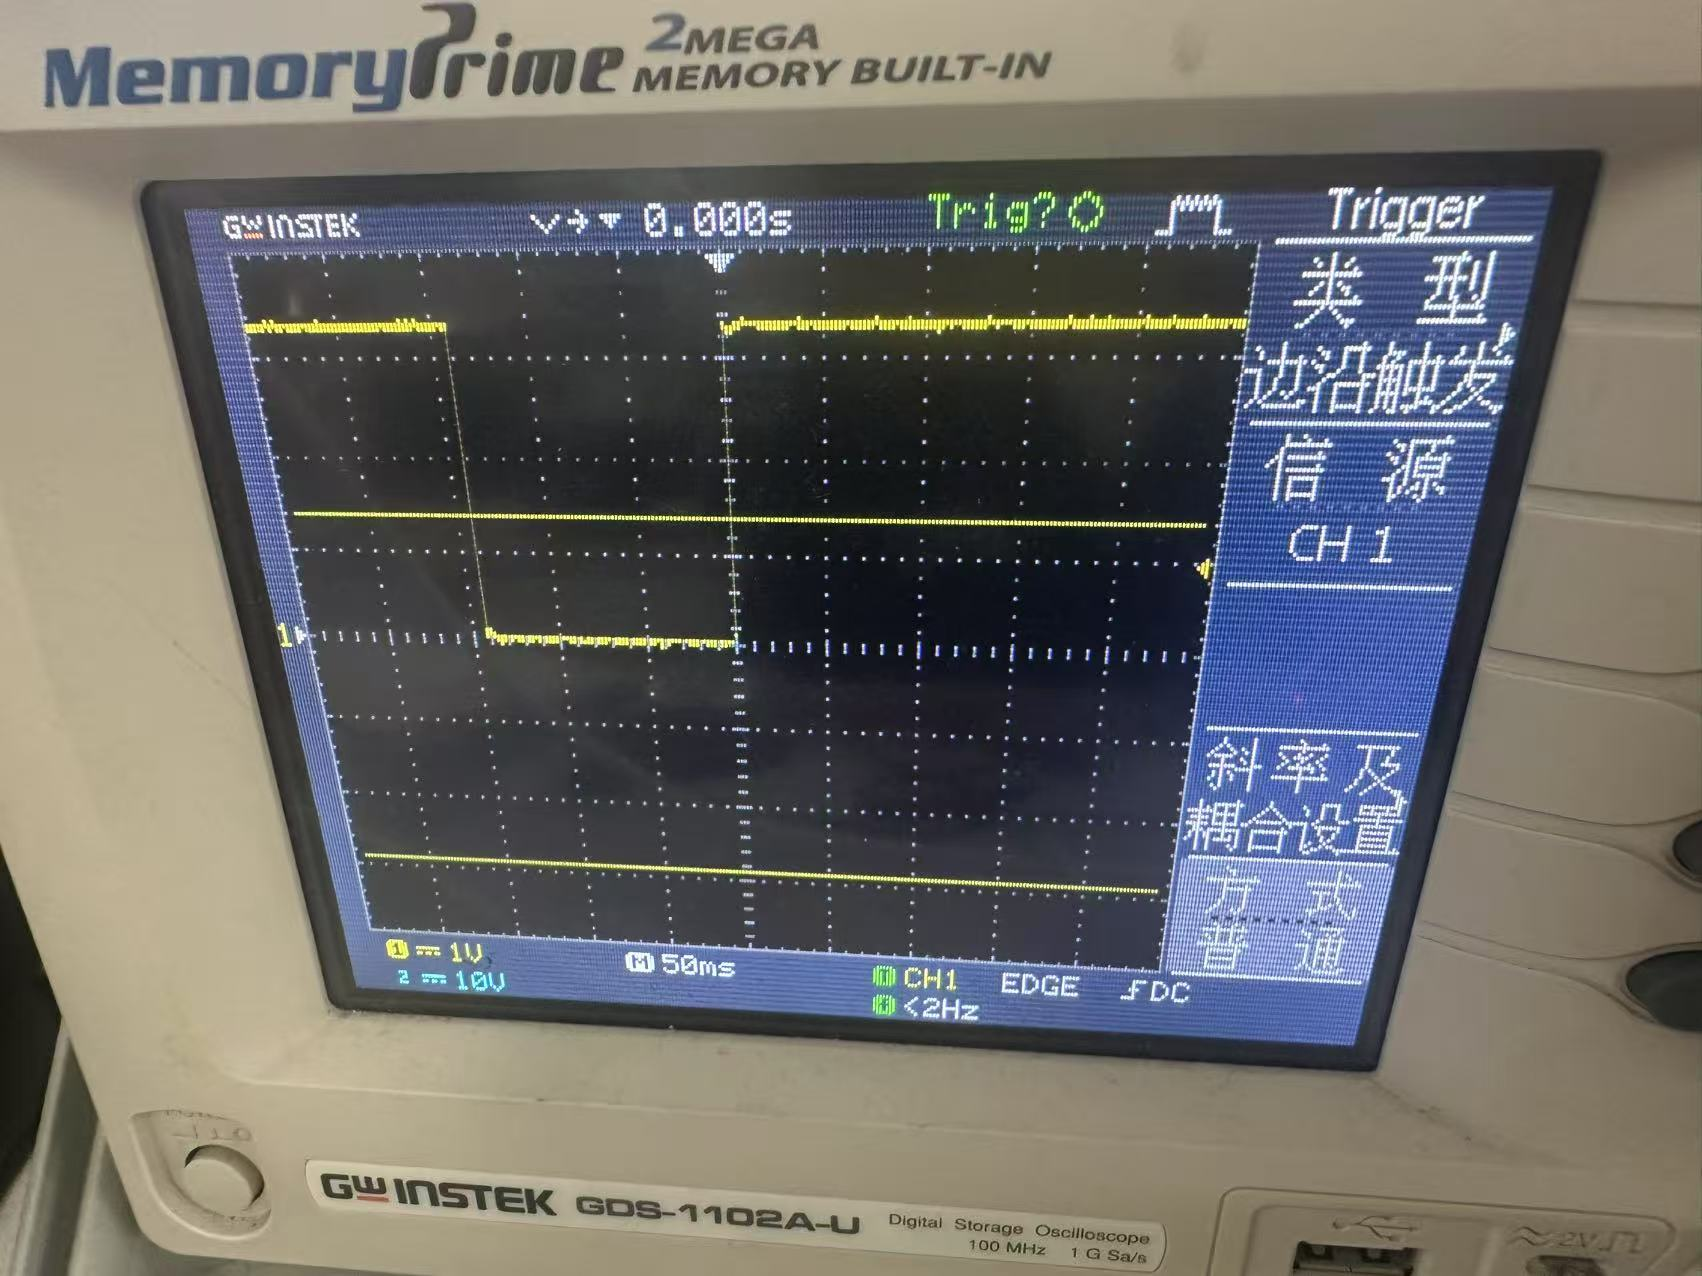
\includegraphics[width=0.9\textwidth]{figures/key5.jpg}
      \caption{无毛刺按压结果}
  \end{minipage}%
  \begin{minipage}[b]{0.5\linewidth}
      \centering
      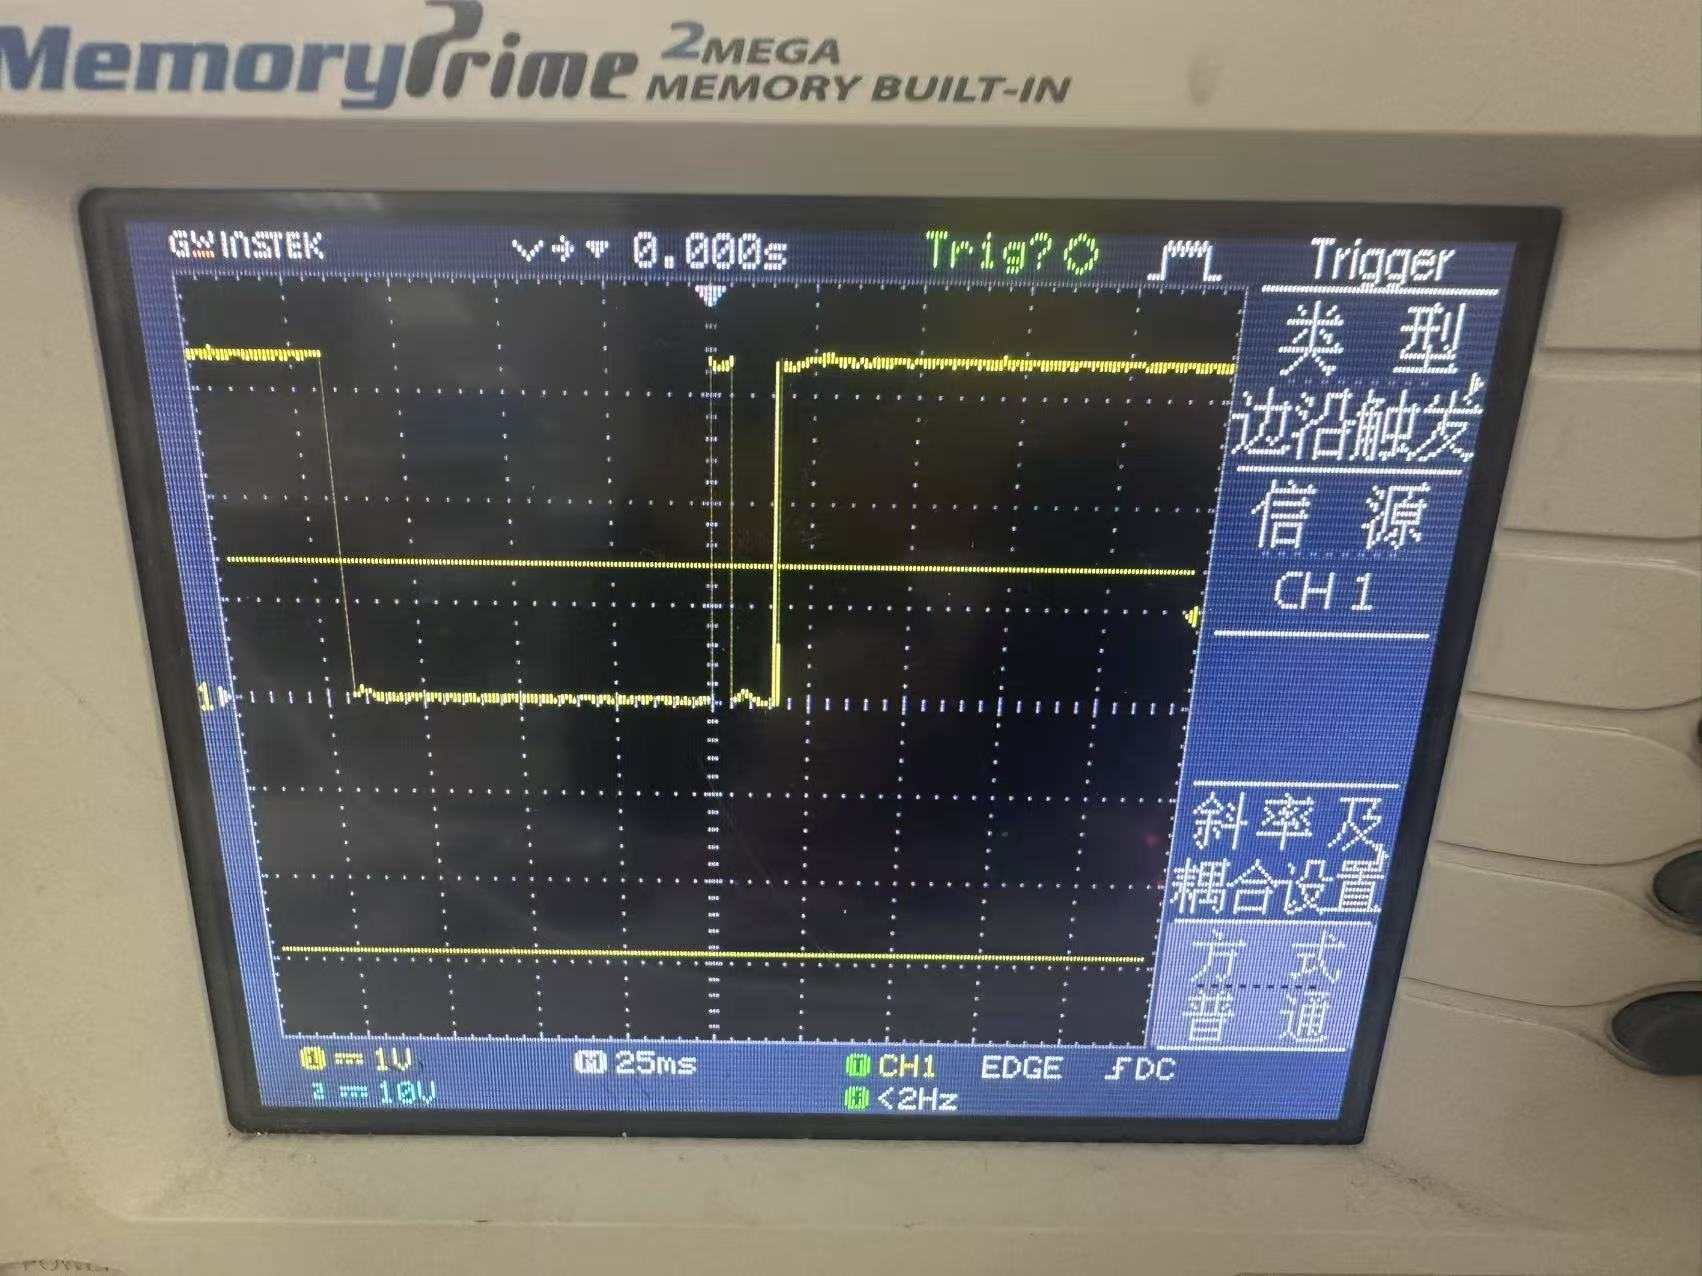
\includegraphics[width=0.9\textwidth]{figures/key4.jpg}
      \caption{有毛刺按压结果}
  \end{minipage}
\end{figure}

\subsubsection{步骤3}

【实验要求】：
修改该程序
key\_in.ino
，使修改后的程序能准
确地读取并记录下以各种按键速度连续按键的次数
（注：每“按下
放开”只能算一次按键）

【代码段与实验结果】：
如图，经修改后，程序能准
确地读取并记录下以各种按键速度连续按键的次数，虽然此时还未处理毛刺问题，但或许由于按钮机械性能较好，对
各种速度/连续按键处理已然较好
\begin{figure}[H]
  \centering
  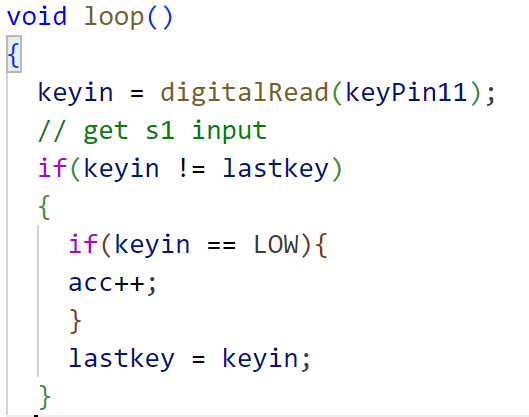
\includegraphics[width=0.7\linewidth]{figures/key1.png} % 数字表示放缩比例
  \caption{软硬件联调任务四代码}
\end{figure}

\subsubsection{步骤4}

【实验要求】：
毛刺由于按键的机械特性而存在。会造成键被误按。
常规的去除毛刺方法是在产生毛刺其间暂停对按键信号的读入，这
可以用恰当的软件延时来实现。
但软件延时过量又会造成对按键响应的迟钝。
调试软件使其既能避免毛刺，又能对按键由恰当的及时正
确的反应，是一个好键盘的终极最求，需要在按键系统调
试过程中结合硬件特性，对软件仔细调教

【代码段与实验结果】：通过在loop()中添加消抖函数，忽略小于宏DEBOUNCE\_DELAY的毛刺，实现对毛刺的过滤，
同时增加[DEBUG]输出，使得不必每一次都通过“r”获取次数，更加直观明了

\begin{figure}[H]
  \centering
  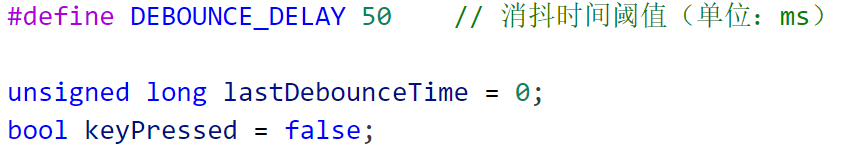
\includegraphics[width=1\linewidth]{figures/key2.png} % 数字表示放缩比例
  \caption{软硬件联调任务四代码}
\end{figure}

\begin{figure}[H]
  \centering
  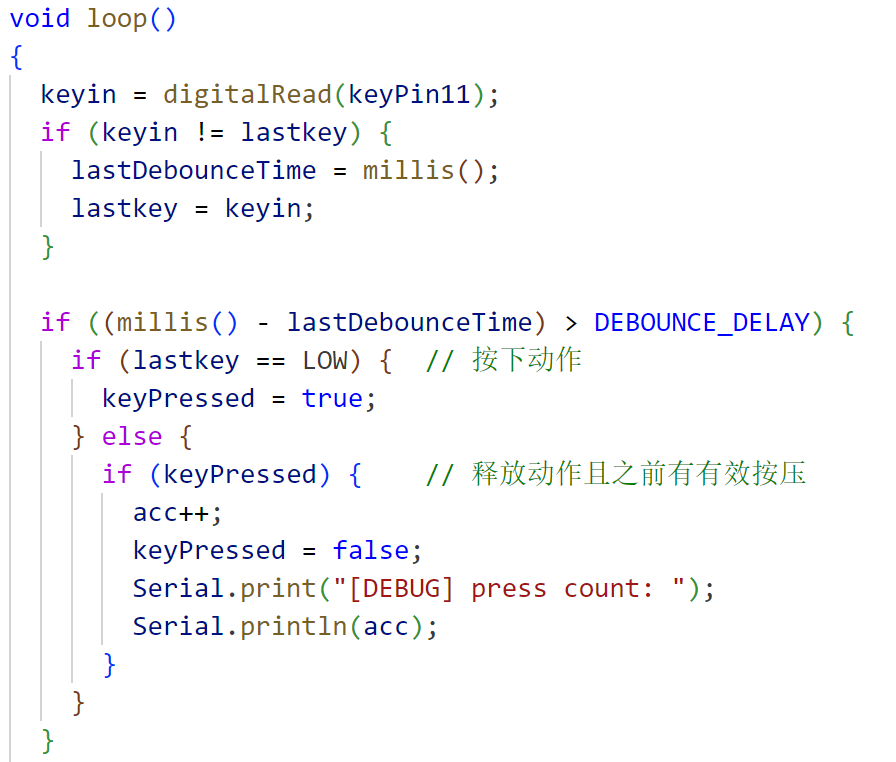
\includegraphics[width=1\linewidth]{figures/key3.png} % 数字表示放缩比例
  \caption{软硬件联调任务四代码}
\end{figure}
\section{系统测试}

\subsection{连接手机}
【测试用例描述】：
\begin{enumerate}
  \item 使用安卓手机，关闭移动网络流量，开放热点(热点名,密码由英文字母和数字组成)，AP频段设置在2.4GHz频段上
  \item 在程序中设置ssid和password与手机热点相符，将程序烧入板子中
  \item 运行智能插座小程序，使得手机与智能插座连接
\end{enumerate}

【测试目的】：验证智能插座可连一个手机

【测试过程及其结果】：手机与智能插座连接成功

\begin{figure}[H]
  \centering
  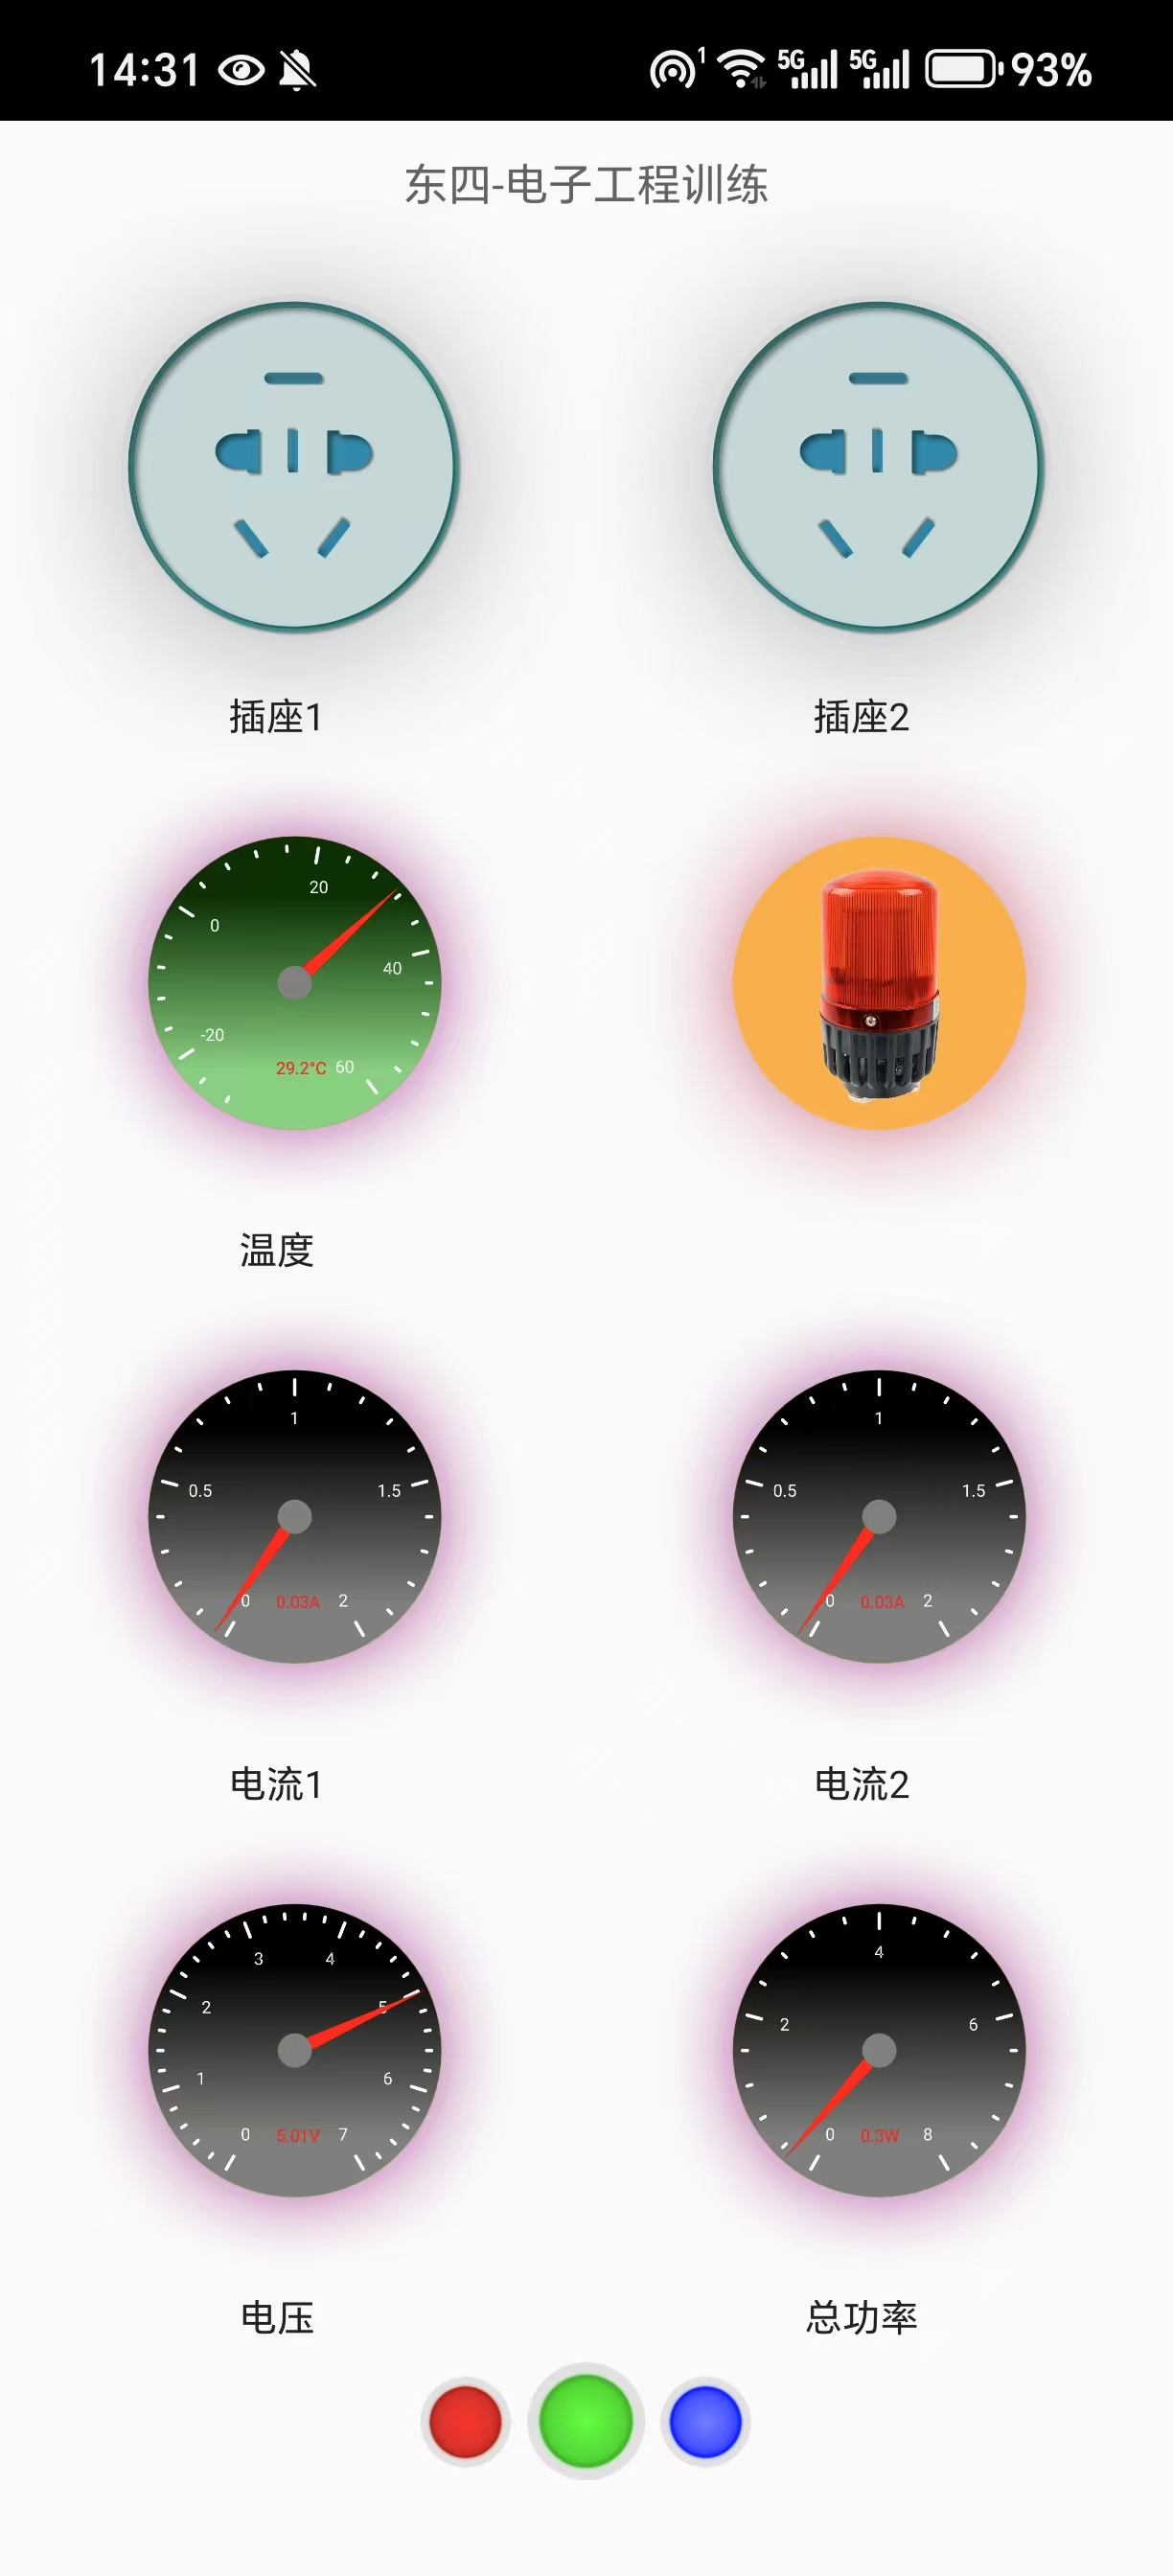
\includegraphics[width=0.25\linewidth]{figures/sys1.jpg} % 数字表示放缩比例
  \caption{连接手机成功}
\end{figure}

\subsection{插座开关手动控制，以及温度、电压、电流和功率显示}

【测试用例描述】
\begin{enumerate}
  \item 将小台灯插在插座1上
  \item 手动打开插座1，观察继电器与发光二极管D1状态
  \item 在智能插座App读取对应的温度、电压、电流和功率
  \item 将风扇插到插座2上，并更换不同的挡位，重复步骤（2）（3）

\end{enumerate}

【测试目的】：验证插座开关手动控制，以及温度、电压、电流和功率显示功能

【测试过程及其结果】：插座1与插座2通路均能正常连通，继电器发出咔哒声响闭合，发光二极管亮起

【附图】：
\begin{figure}[H]
  \centering
  \begin{minipage}[b]{0.25\linewidth}
    \centering
    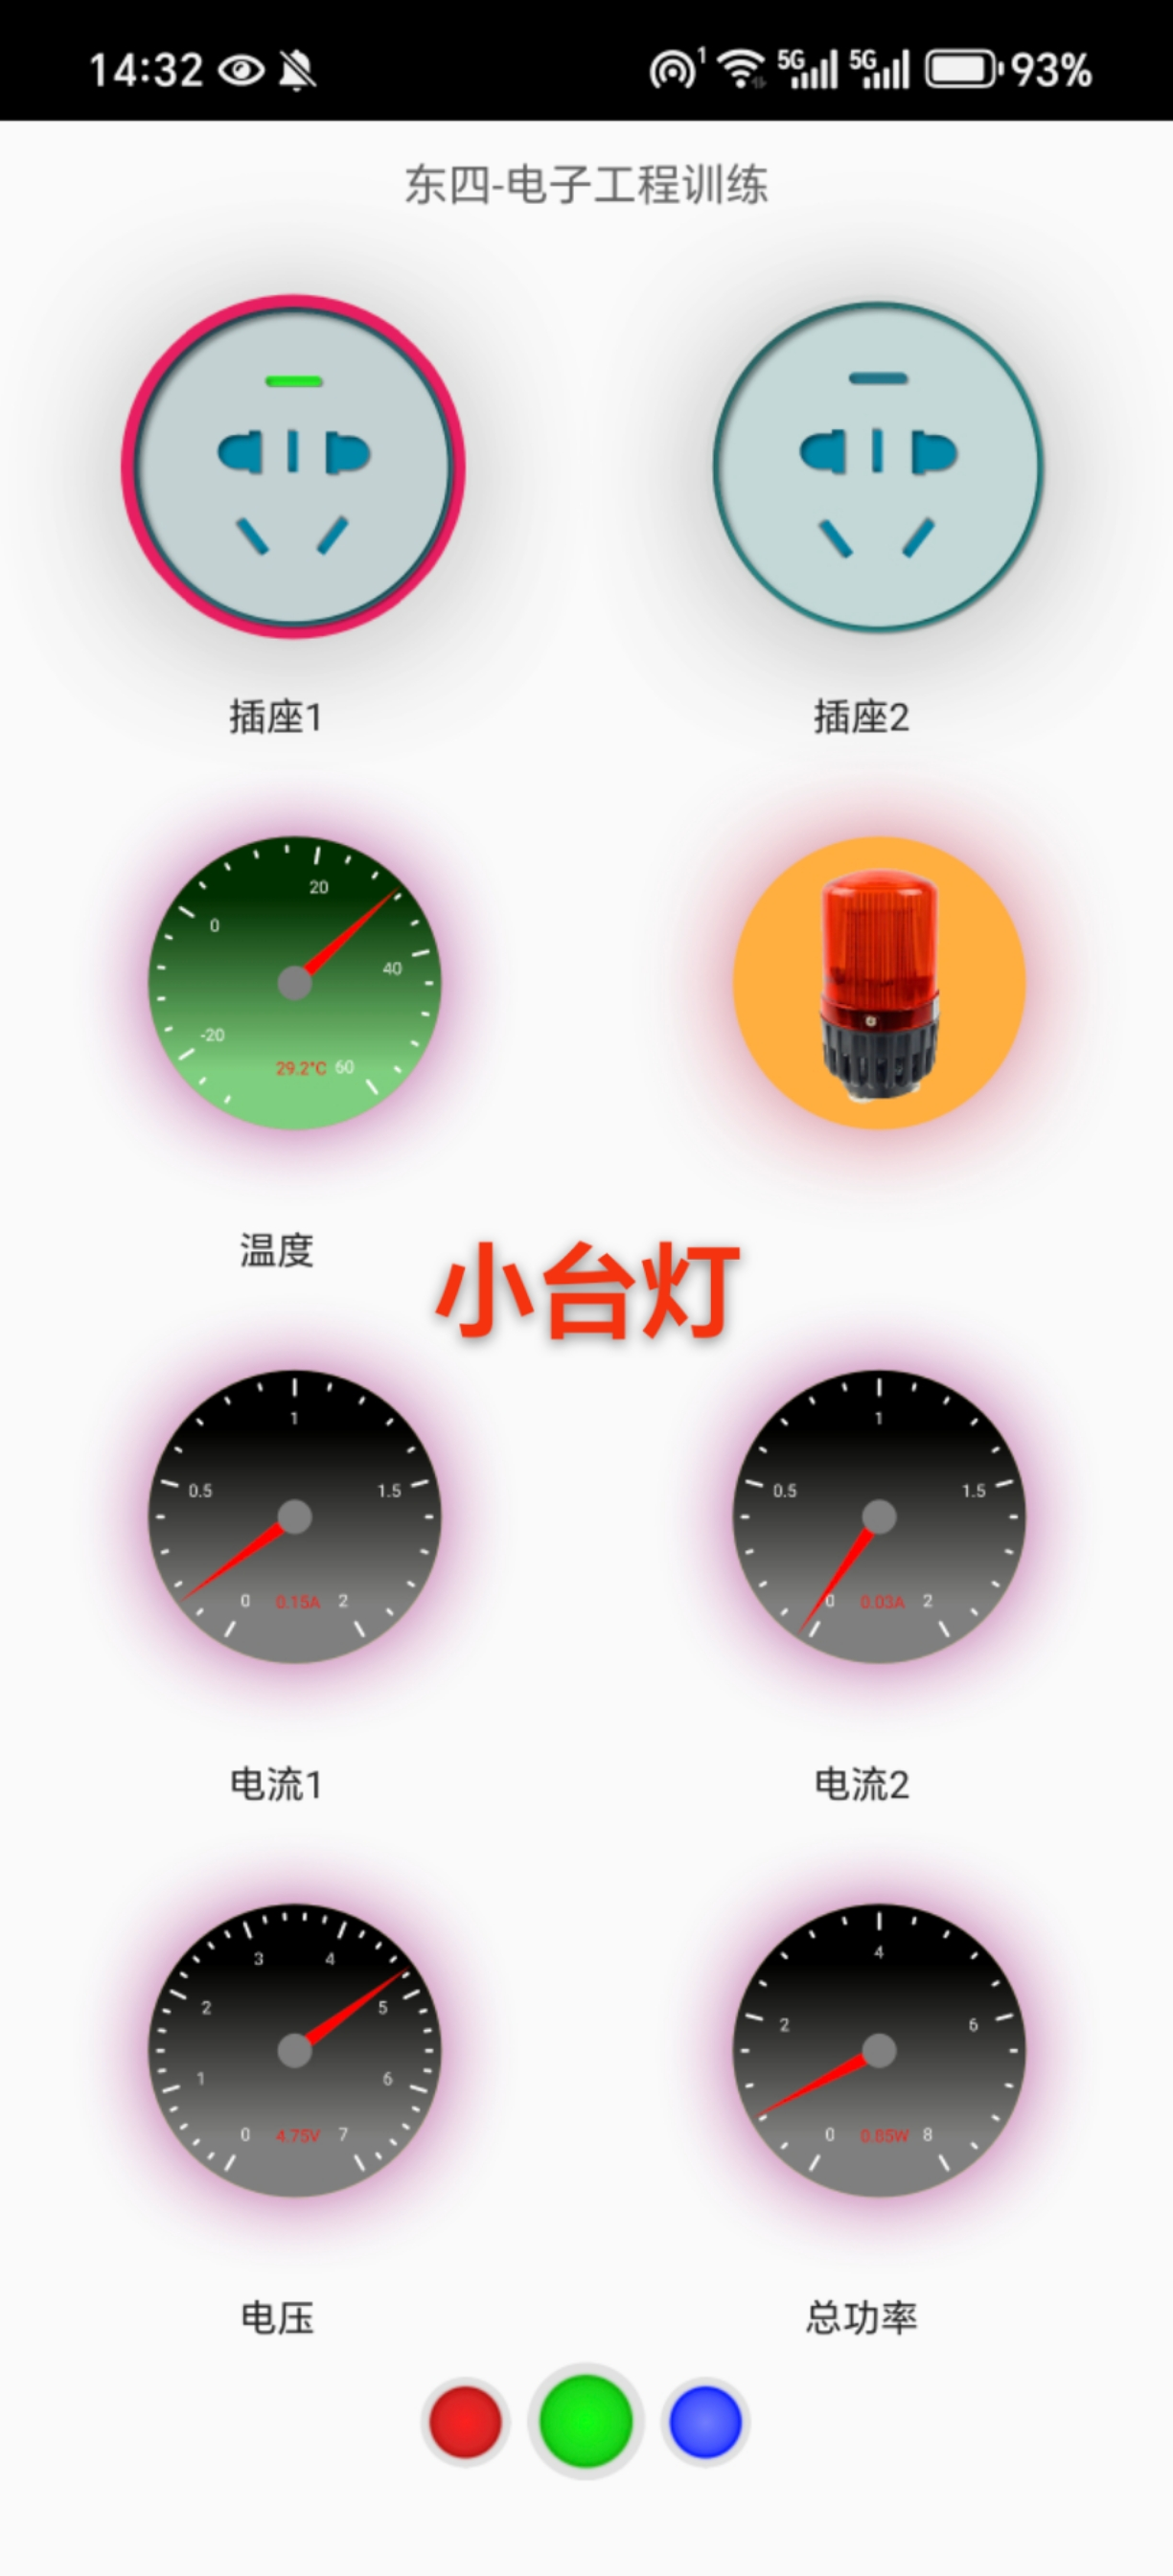
\includegraphics[width=0.9\textwidth]{figures/light.jpg}
    \caption{小台灯}
  \end{minipage}%
  \begin{minipage}[b]{0.25\linewidth}
    \centering
    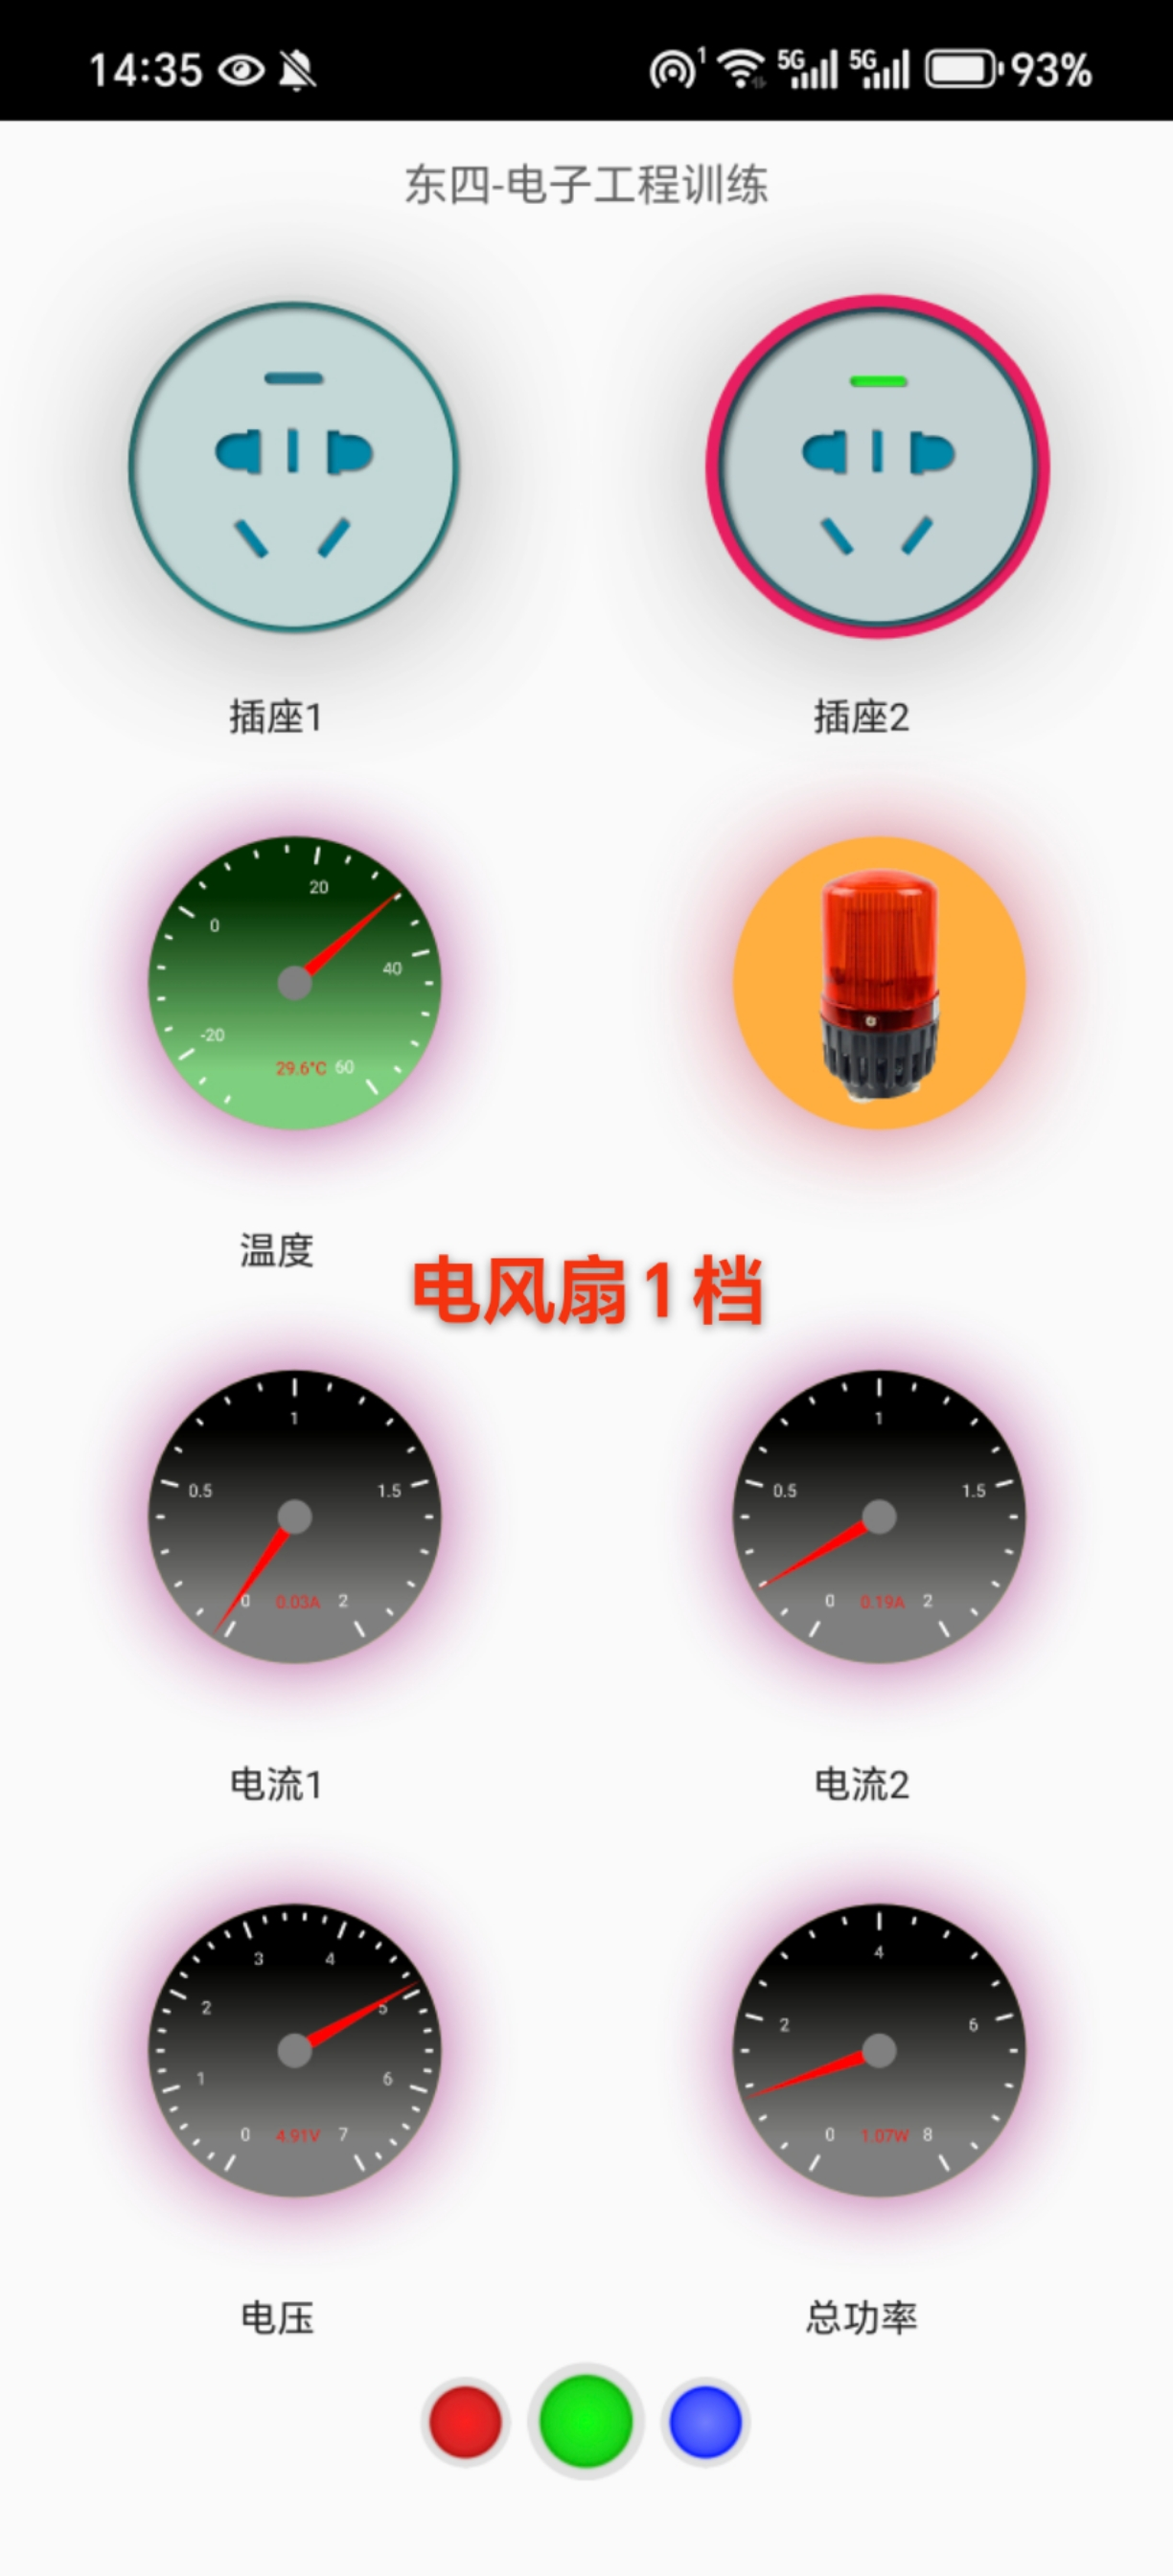
\includegraphics[width=0.9\textwidth]{figures/fan1.jpg}
    \caption{电风扇1档}
  \end{minipage}%
  \begin{minipage}[b]{0.25\linewidth}
    \centering
    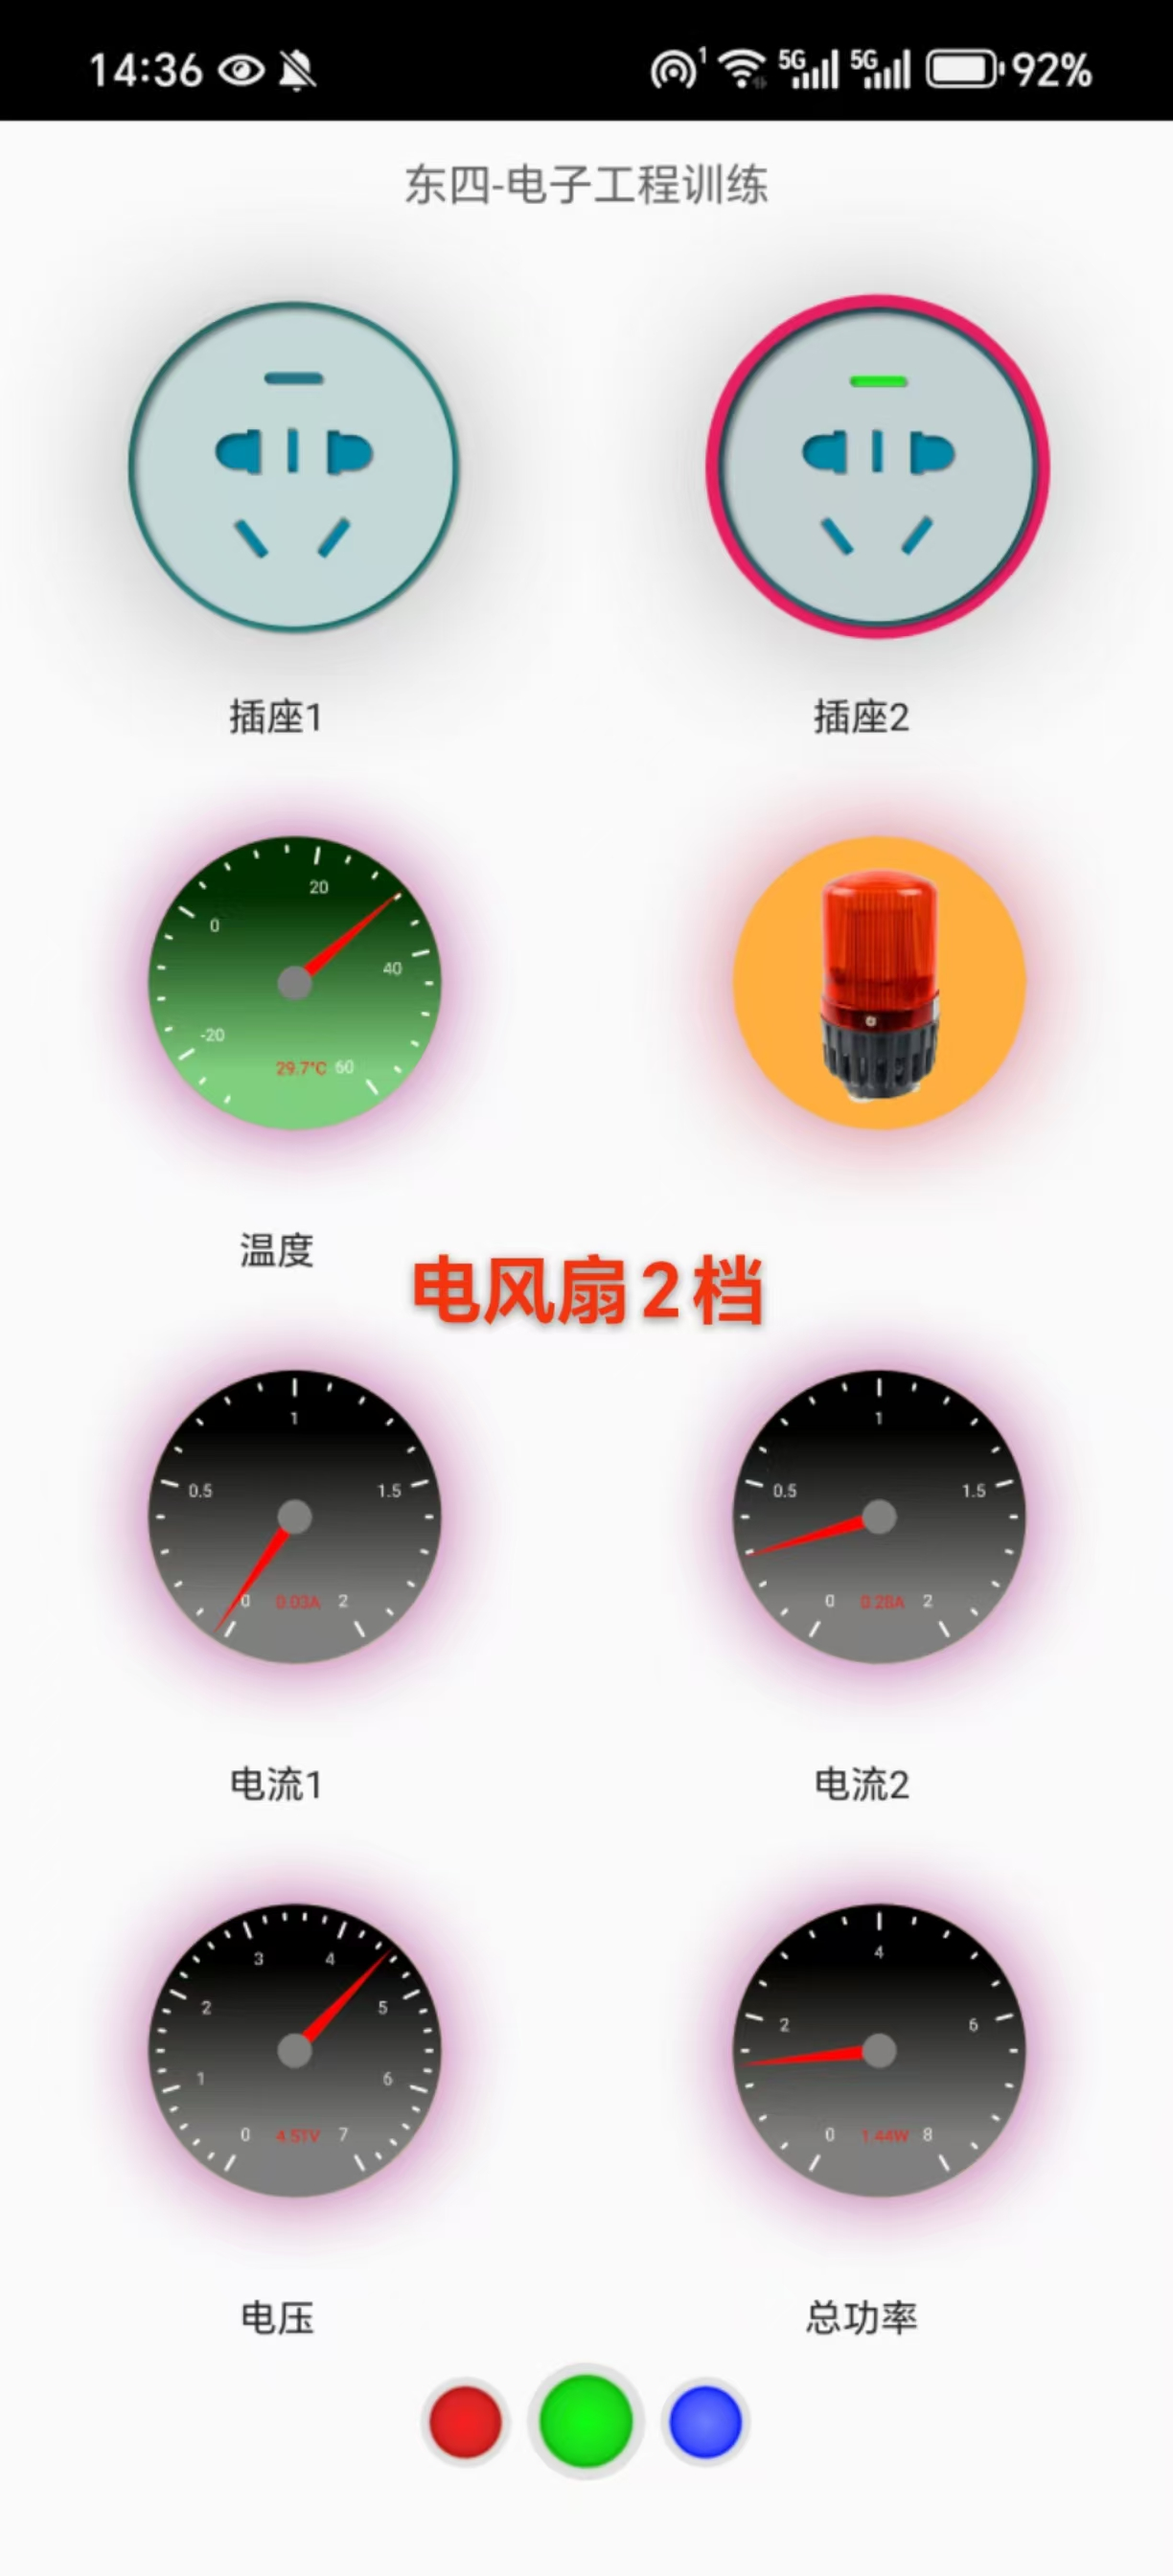
\includegraphics[width=0.9\textwidth]{figures/fan2.jpg}
    \caption{电风扇2档}
  \end{minipage}%
  \begin{minipage}[b]{0.25\linewidth}
    \centering
    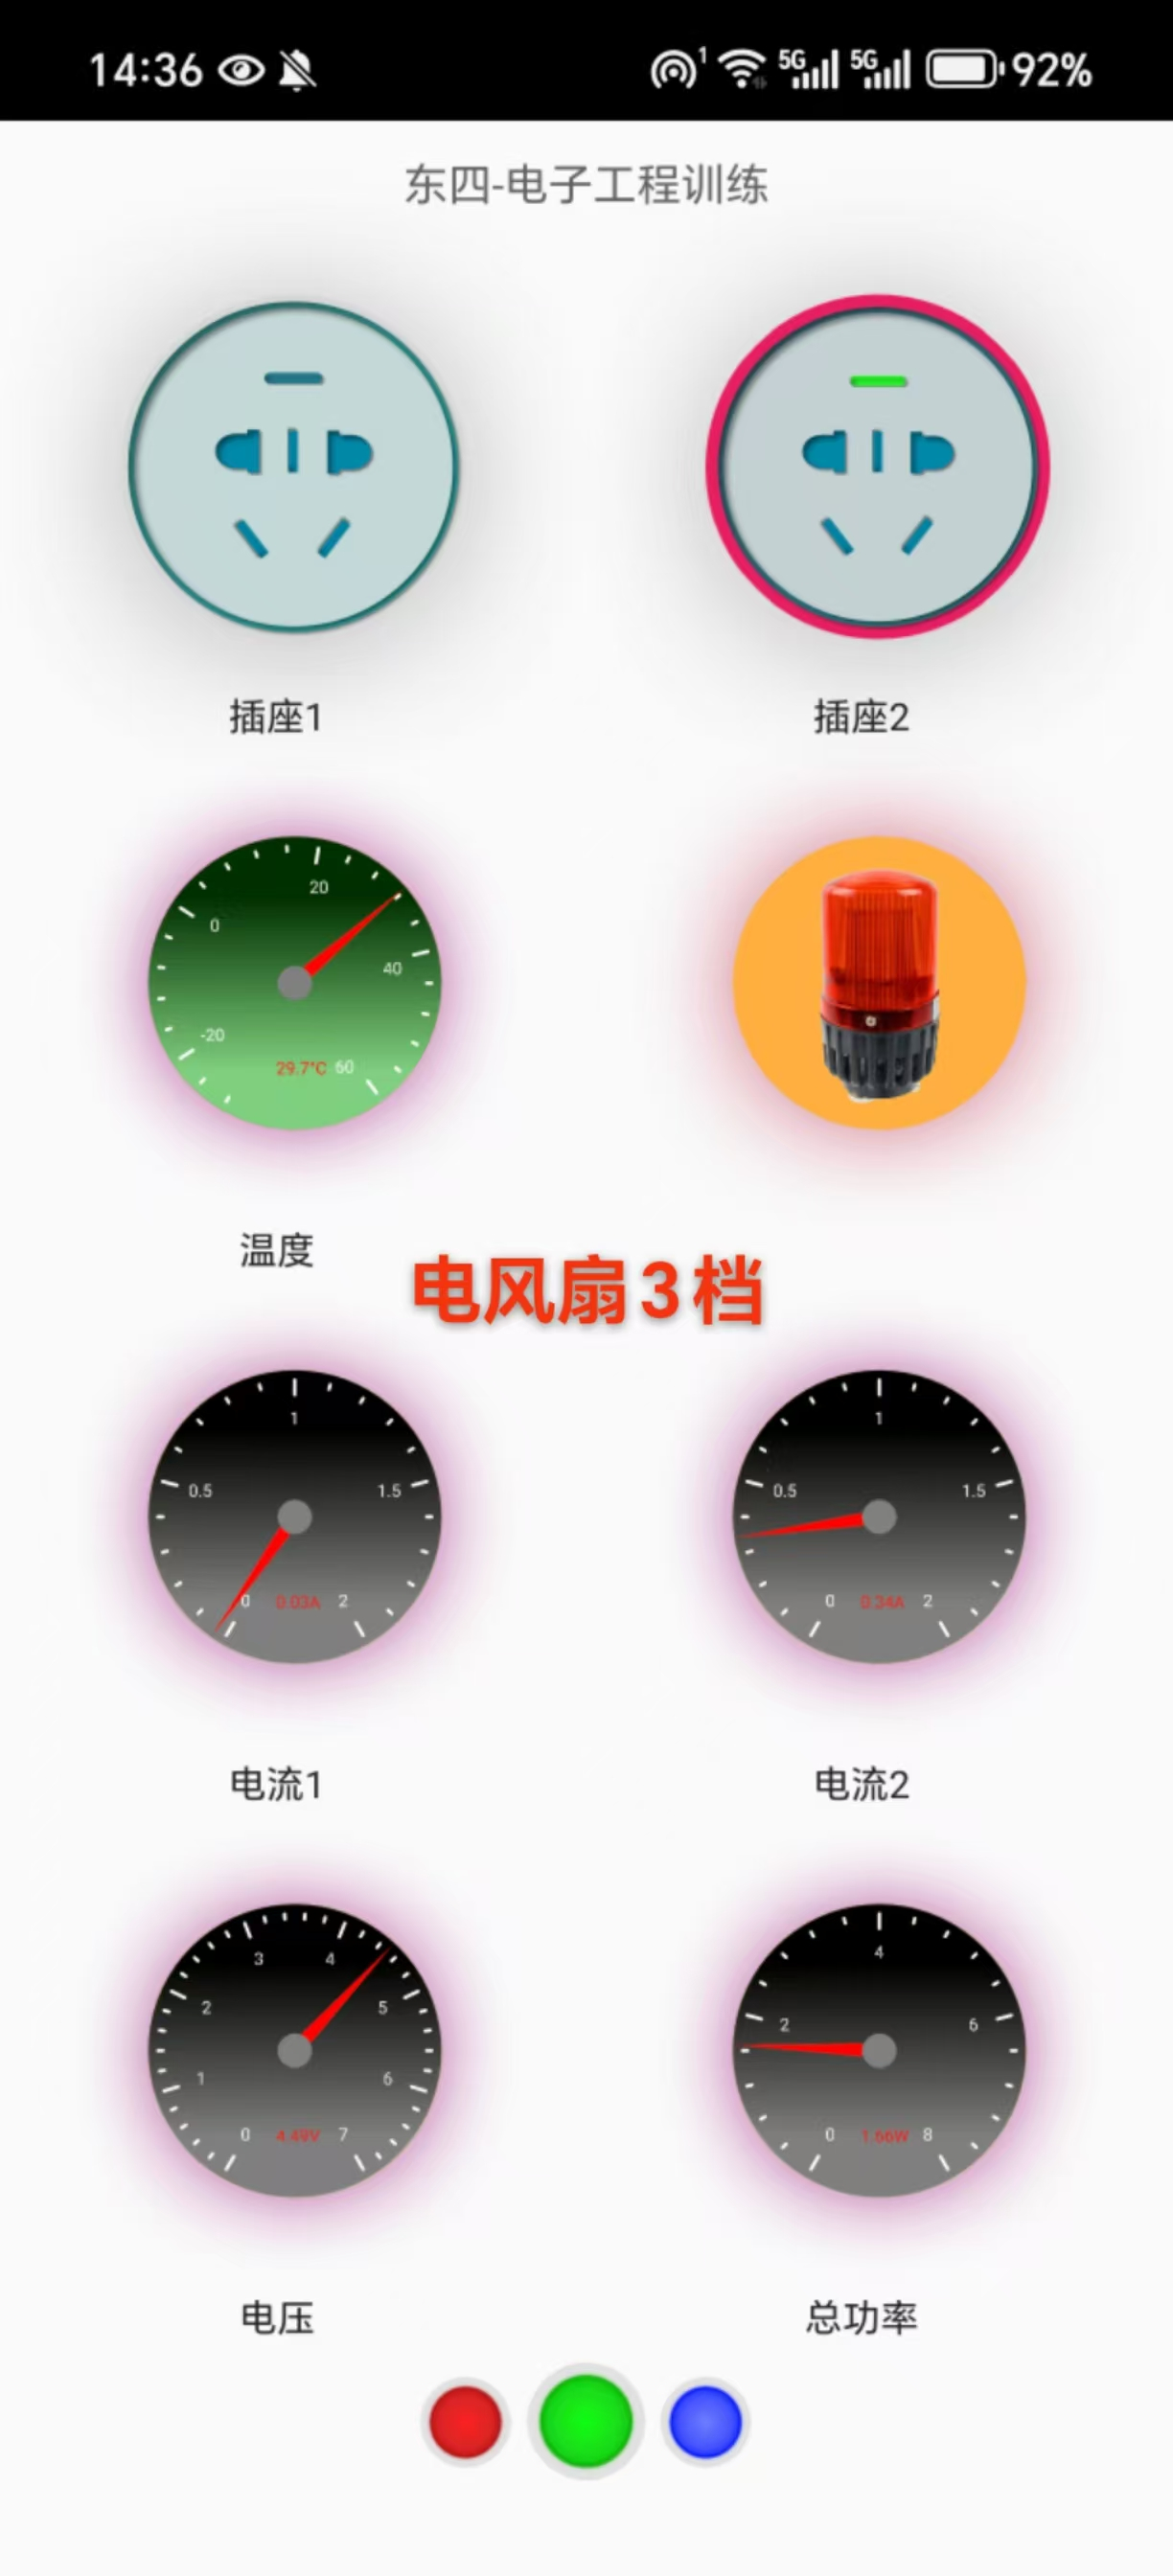
\includegraphics[width=0.9\textwidth]{figures/fan3.jpg}
    \caption{电风扇3档}
  \end{minipage}
\end{figure}
\subsection{定时开/关，延时开/关}
\subsubsection{定时开关}

【测试用例描述】：
\begin{enumerate}
  \item 将小台灯插在插座1上，关闭插座1电源
  \item 14：40在智能插座App上设置定时14：41开，预期14：41小台灯亮起
  \item 14：41在智能插座App上设置定时14：42关，预期14：42小台灯熄灭
\end{enumerate}

【测试目的】：验证插座开关定时开/关功能

【测试过程及其结果】：结果符合测试预期，小台灯在14：41亮起，在14：42熄灭
，插座开关定时开/关功能良好

【发现bug】：定时界面无法设置秒数

【附图】：

\subsubsection{延时开关}
  
【测试用例描述】：
\begin{enumerate}
  \item 将小台灯插在插座1上，关闭插座1电源
  \item 14：45在智能插座App上设置延时1min开，预期14：46小台灯亮起
  \item 14：47在智能插座App上设置延时1min关，预期14：48小台灯熄灭
\end{enumerate}

【测试目的】：验证插座开关延时开/关功能

【测试过程及其结果】：结果符合测试预期，小台灯在14：46亮起，在14：48熄灭
，插座开关延时开/关功能良好

【发现bug】：延时界面无法设置秒数

【附图】：
\begin{figure}[H]
  \centering
  \begin{minipage}[b]{0.25\linewidth}
    \centering
    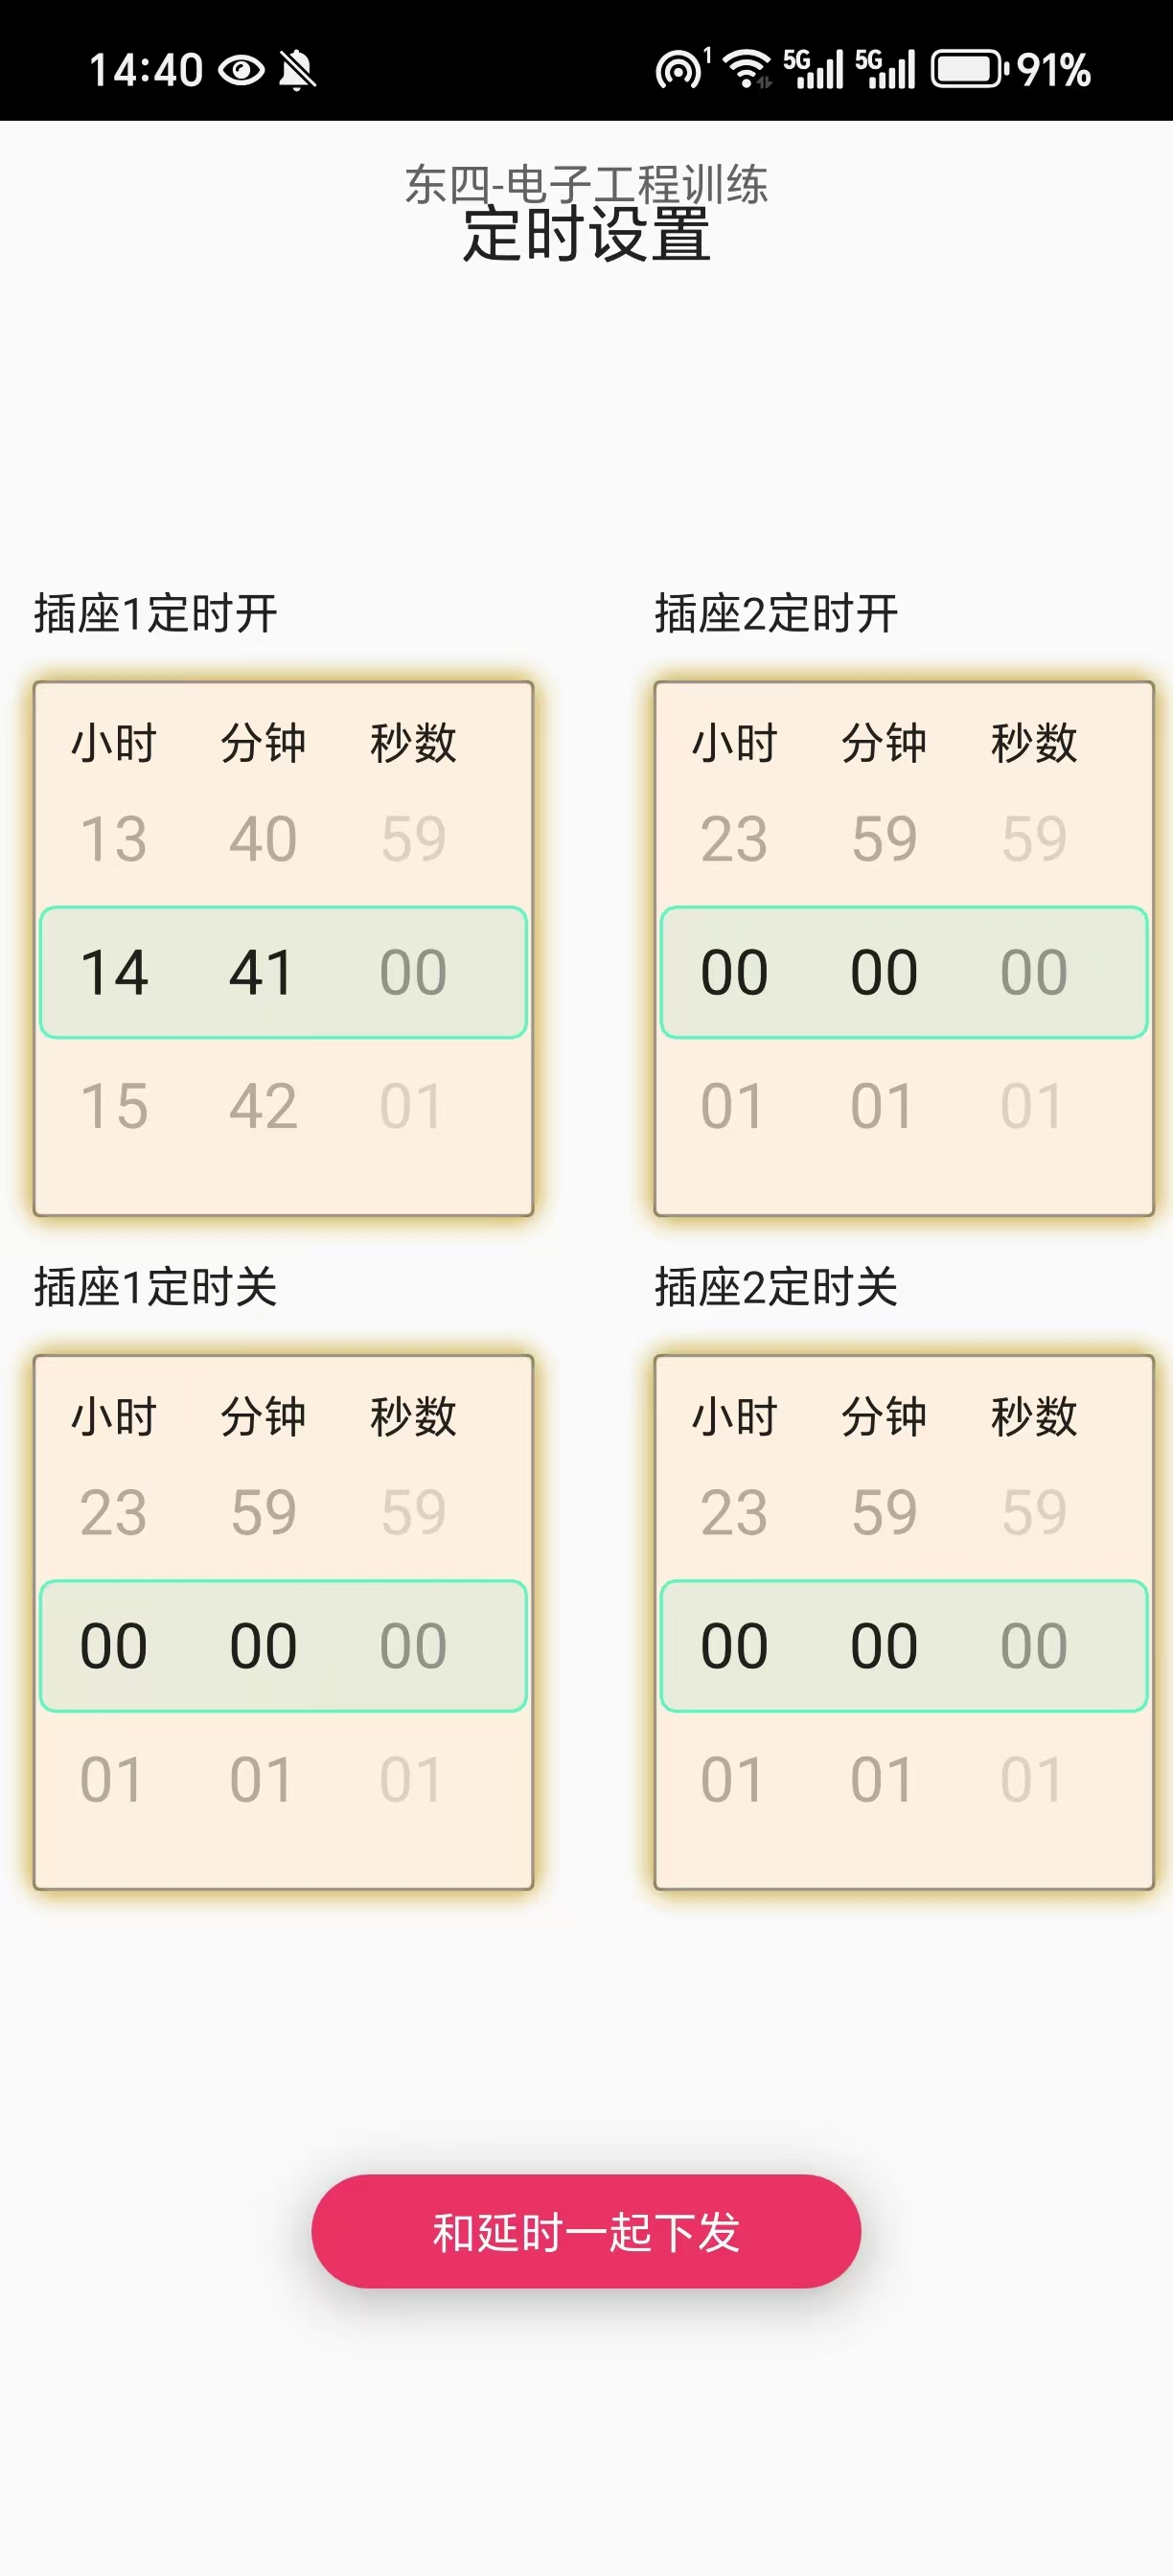
\includegraphics[width=0.9\textwidth]{figures/st.jpg}
    \caption{定时开关}
  \end{minipage}%
  \begin{minipage}[b]{0.25\linewidth}
    \centering
    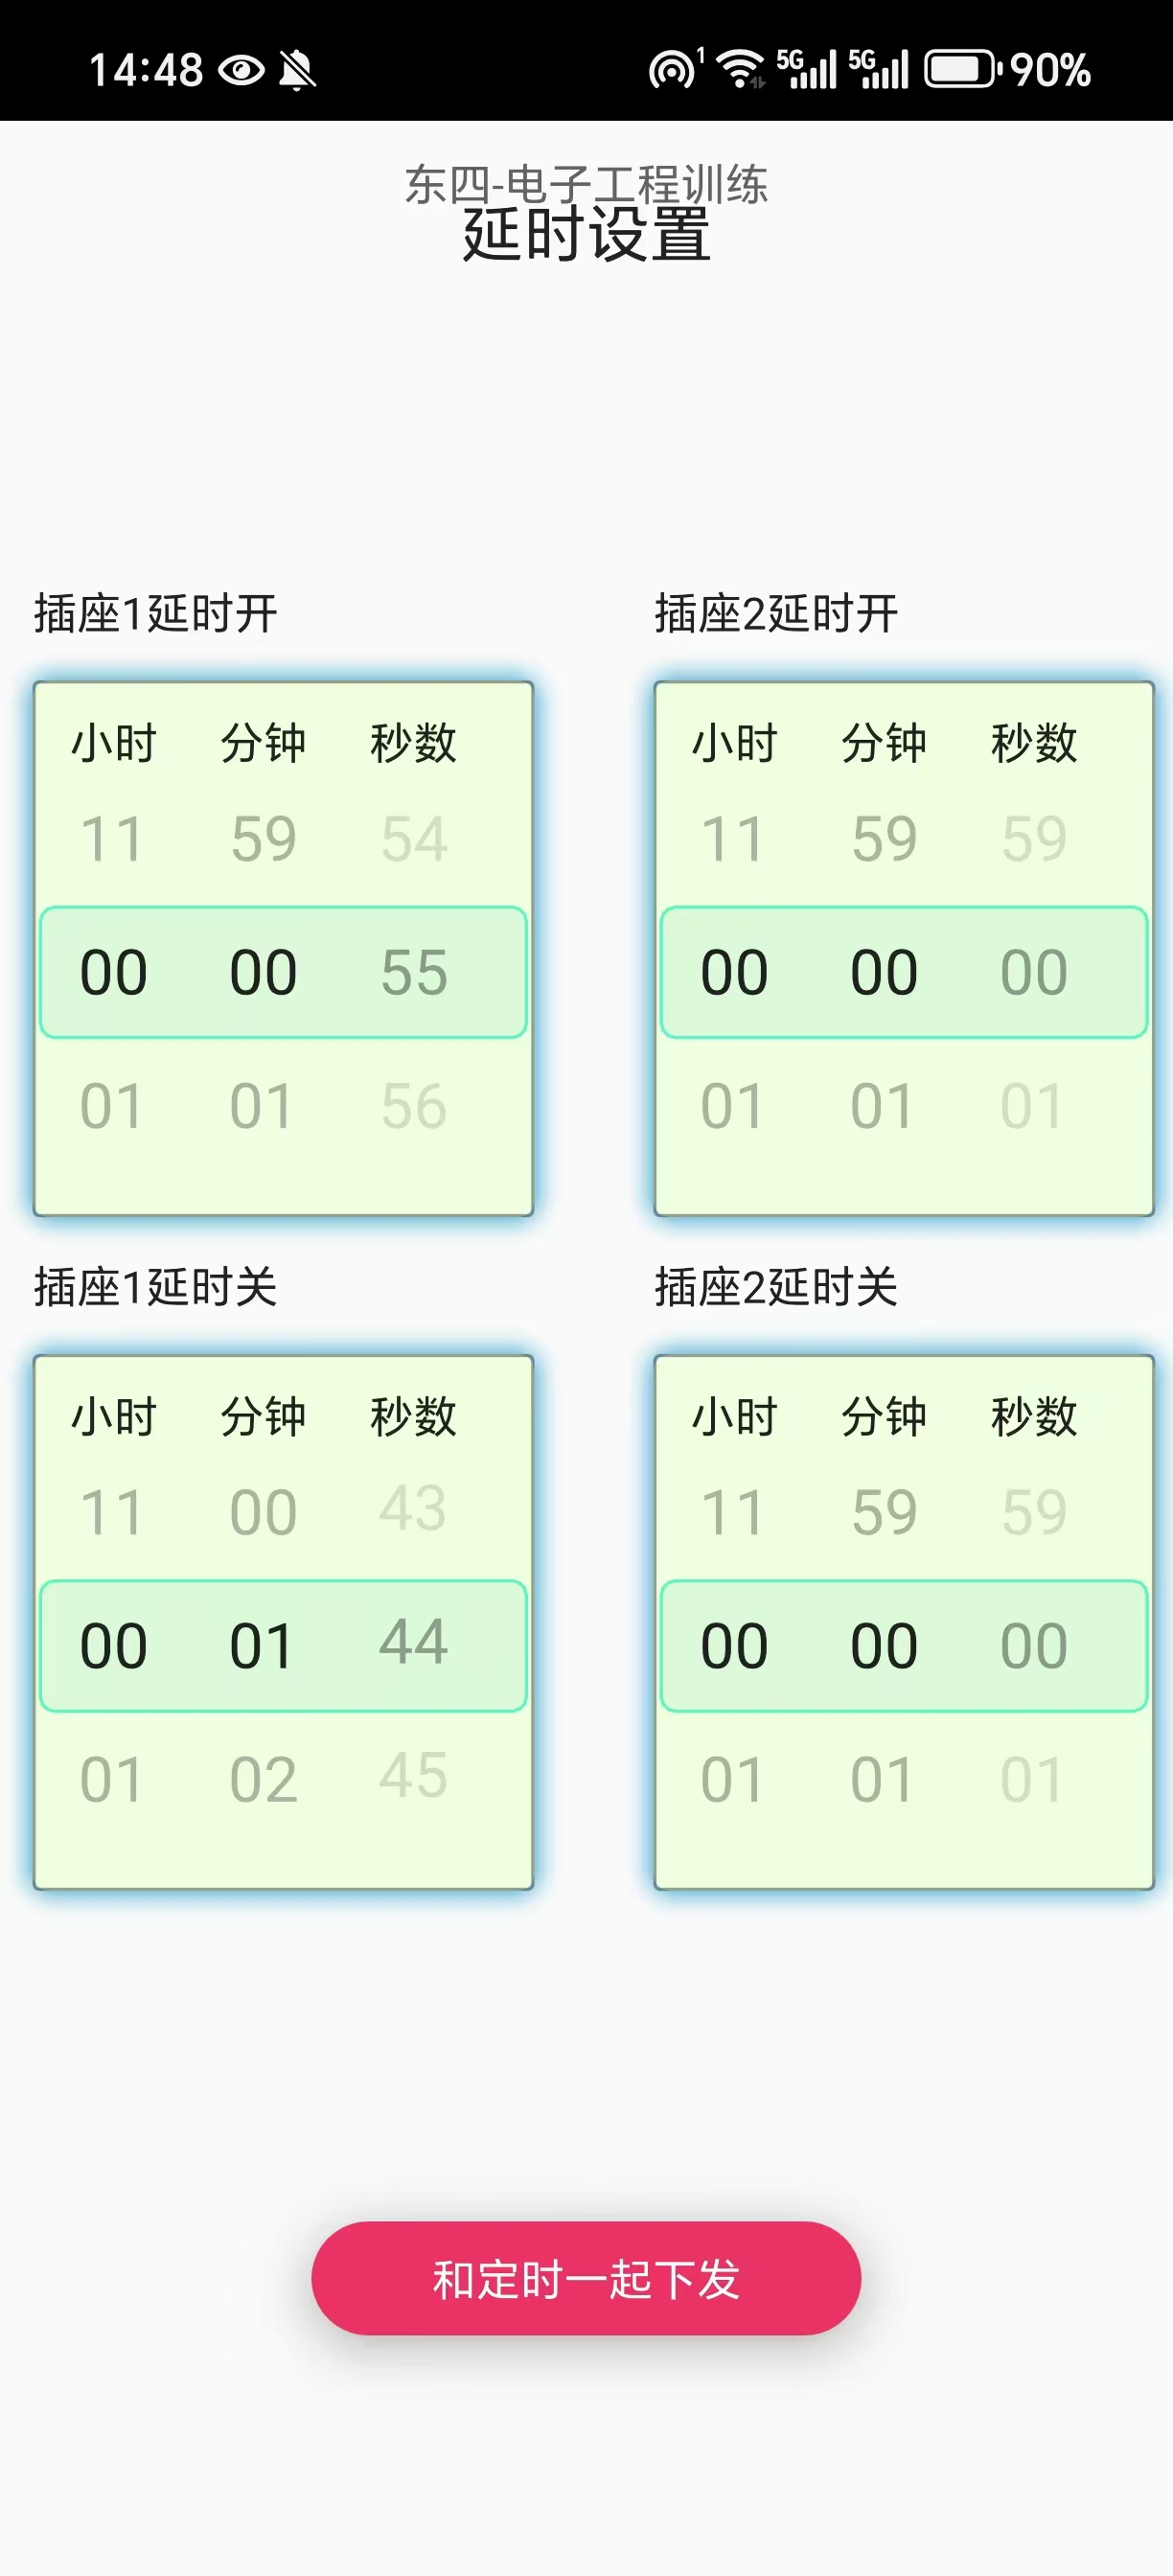
\includegraphics[width=0.9\textwidth]{figures/dt.jpg}
    \caption{延时开关}
  \end{minipage}%
\end{figure}

\subsection{超/欠电压、超电流、超功率、高温/低温告警并自动断开插座供电}
\subsubsection{超电压}

【测试用例描述】：
\begin{enumerate}
  \item 将风扇插在插座1上，关闭插座1电源
  \item 将电压上限设定为4.8V
  \item 开启插座1电源，启动风扇1挡位，预期超电压告警
\end{enumerate}

【测试目的】：测试插座开关超电压报警功能

【测试过程及其结果】：结果符合测试预期，
实时电压在超过4.8V时瞬间报警，
小程序显示电压故障，插座断电，
插座开关超电压报警功能良好

\subsubsection{欠电压}

【测试用例描述】：
\begin{enumerate}
  \item 将风扇插在插座1上，关闭插座1电源
  \item 将电压下限设定为4.5V
  \item 开启插座1电源，启动风扇3挡，预期欠电压告警
\end{enumerate}

【测试目的】：测试插座开关欠电压报警功能

【测试过程及其结果】：结果符合测试预期，
实时电压在低于4.5V时瞬间报警，
小程序显示电压故障，插座断电，
插座开关欠电压报警功能良好

\subsubsection{超电流}

【测试用例描述】：
\begin{enumerate}
  \item 将风扇插在插座1上，关闭插座1电源
  \item 将电流上限设定为0.2A
  \item 开启插座1电源，启动风扇3挡，预期超电流告警
\end{enumerate}

【测试目的】：测试插座开关超电流报警功能

【测试过程及其结果】：结果符合测试预期，
实时电流在超过0.2A时瞬间报警，
小程序显示电流超限，插座断电，
插座开关超电流报警功能良好

【附图】：
\begin{figure}[H]
  \centering
  \begin{minipage}[b]{0.33\linewidth}
    \centering
    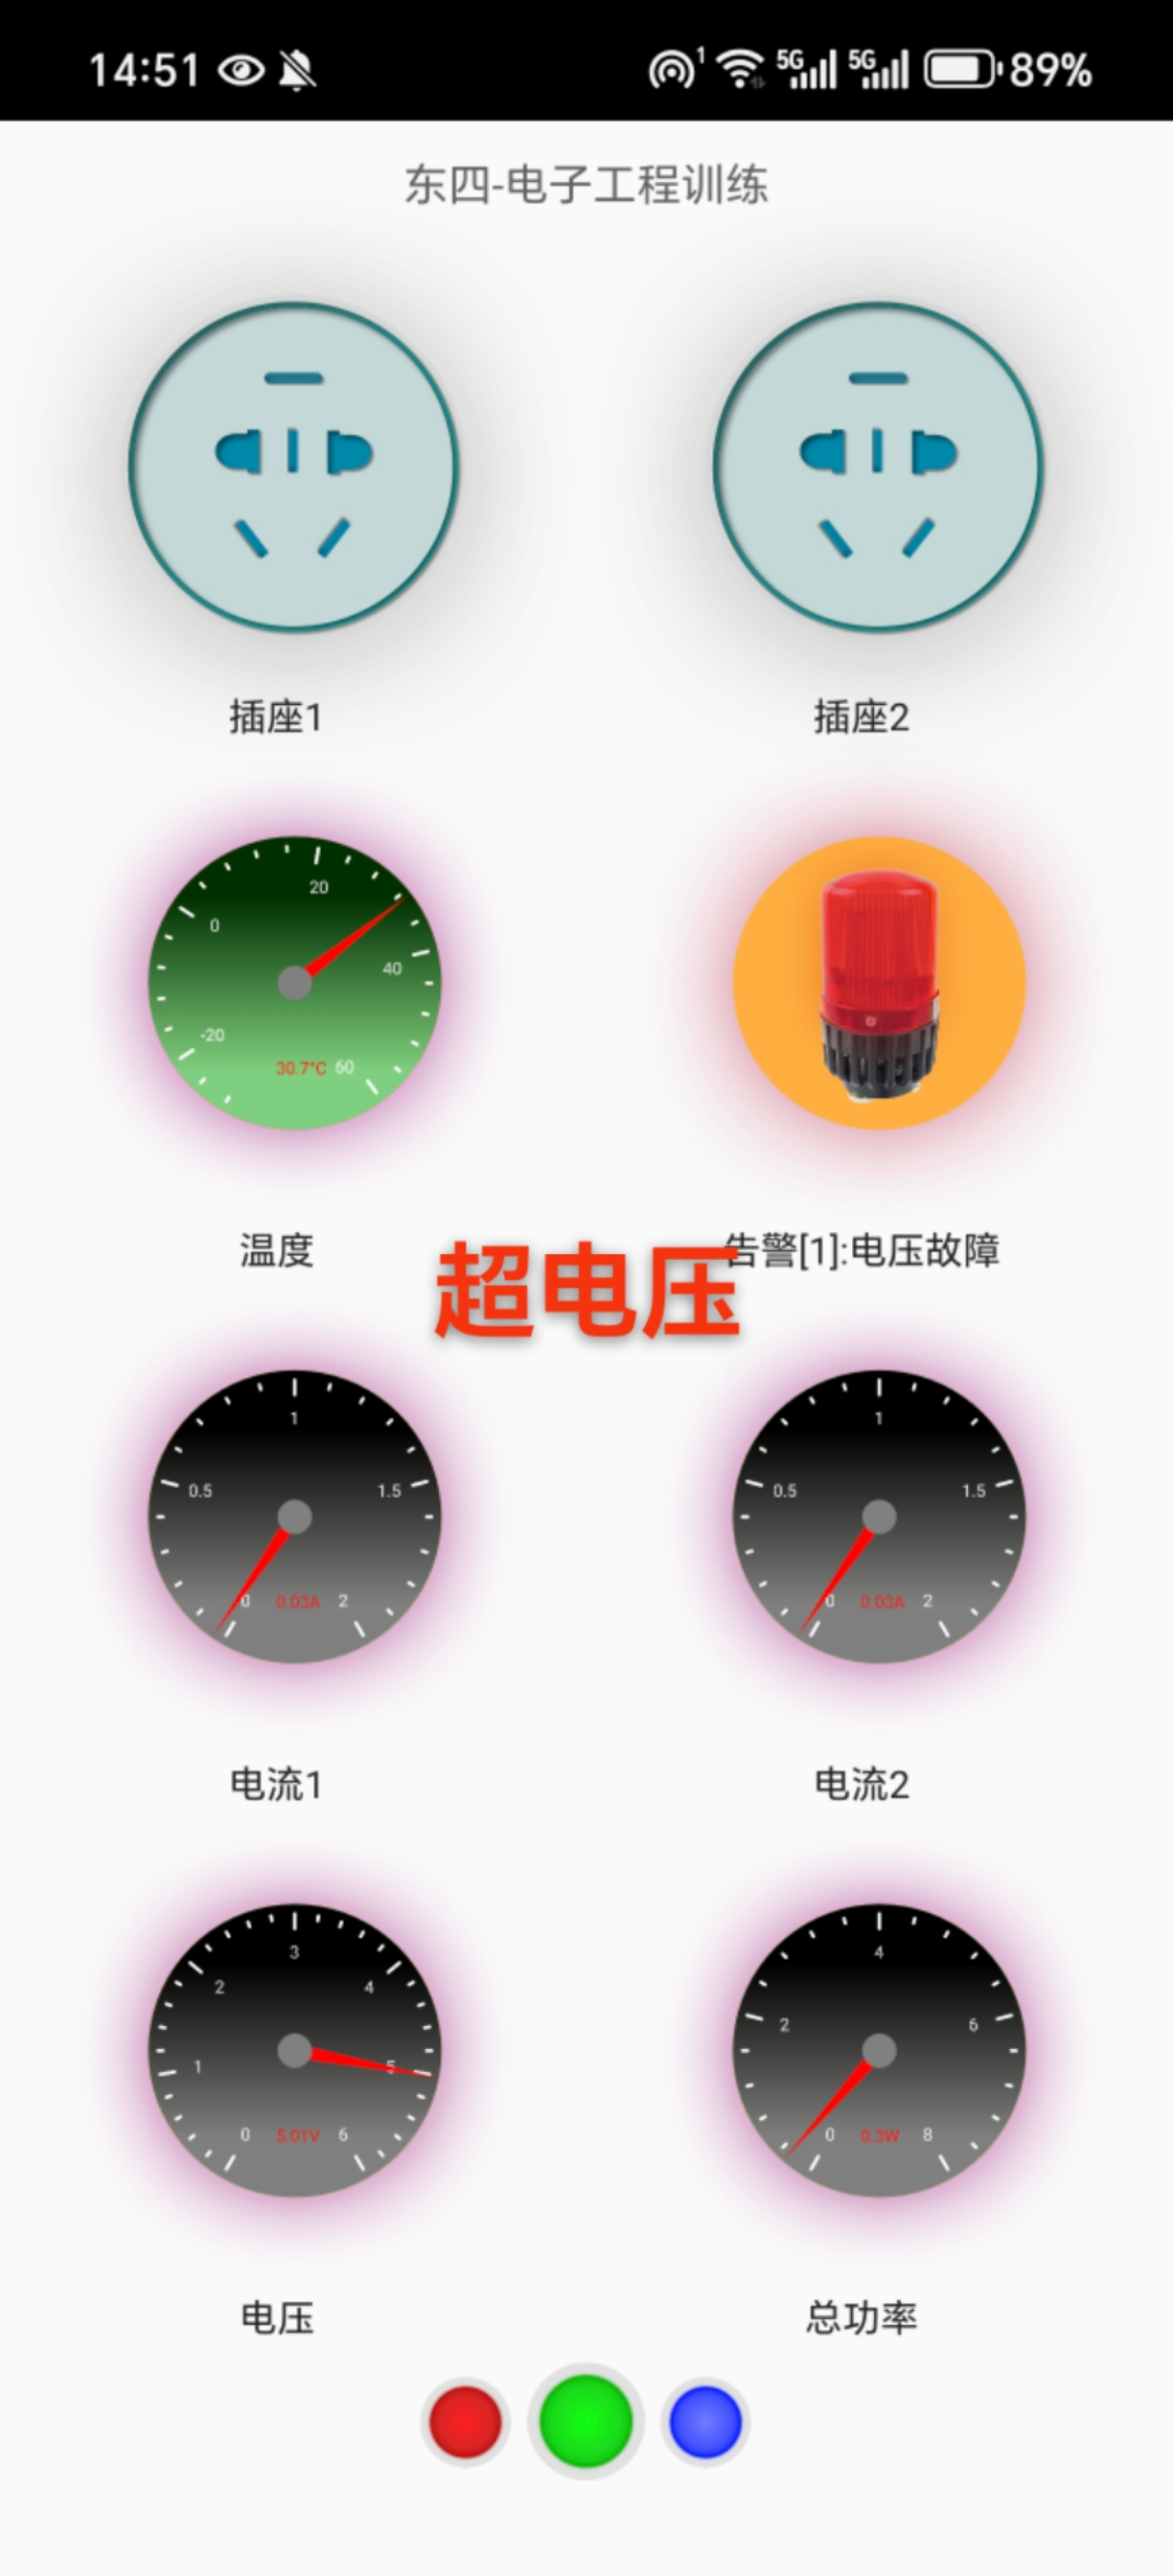
\includegraphics[width=0.9\textwidth]{figures/hv.jpg}
    \caption{超电压}
  \end{minipage}%
  \begin{minipage}[b]{0.33\linewidth}
    \centering
    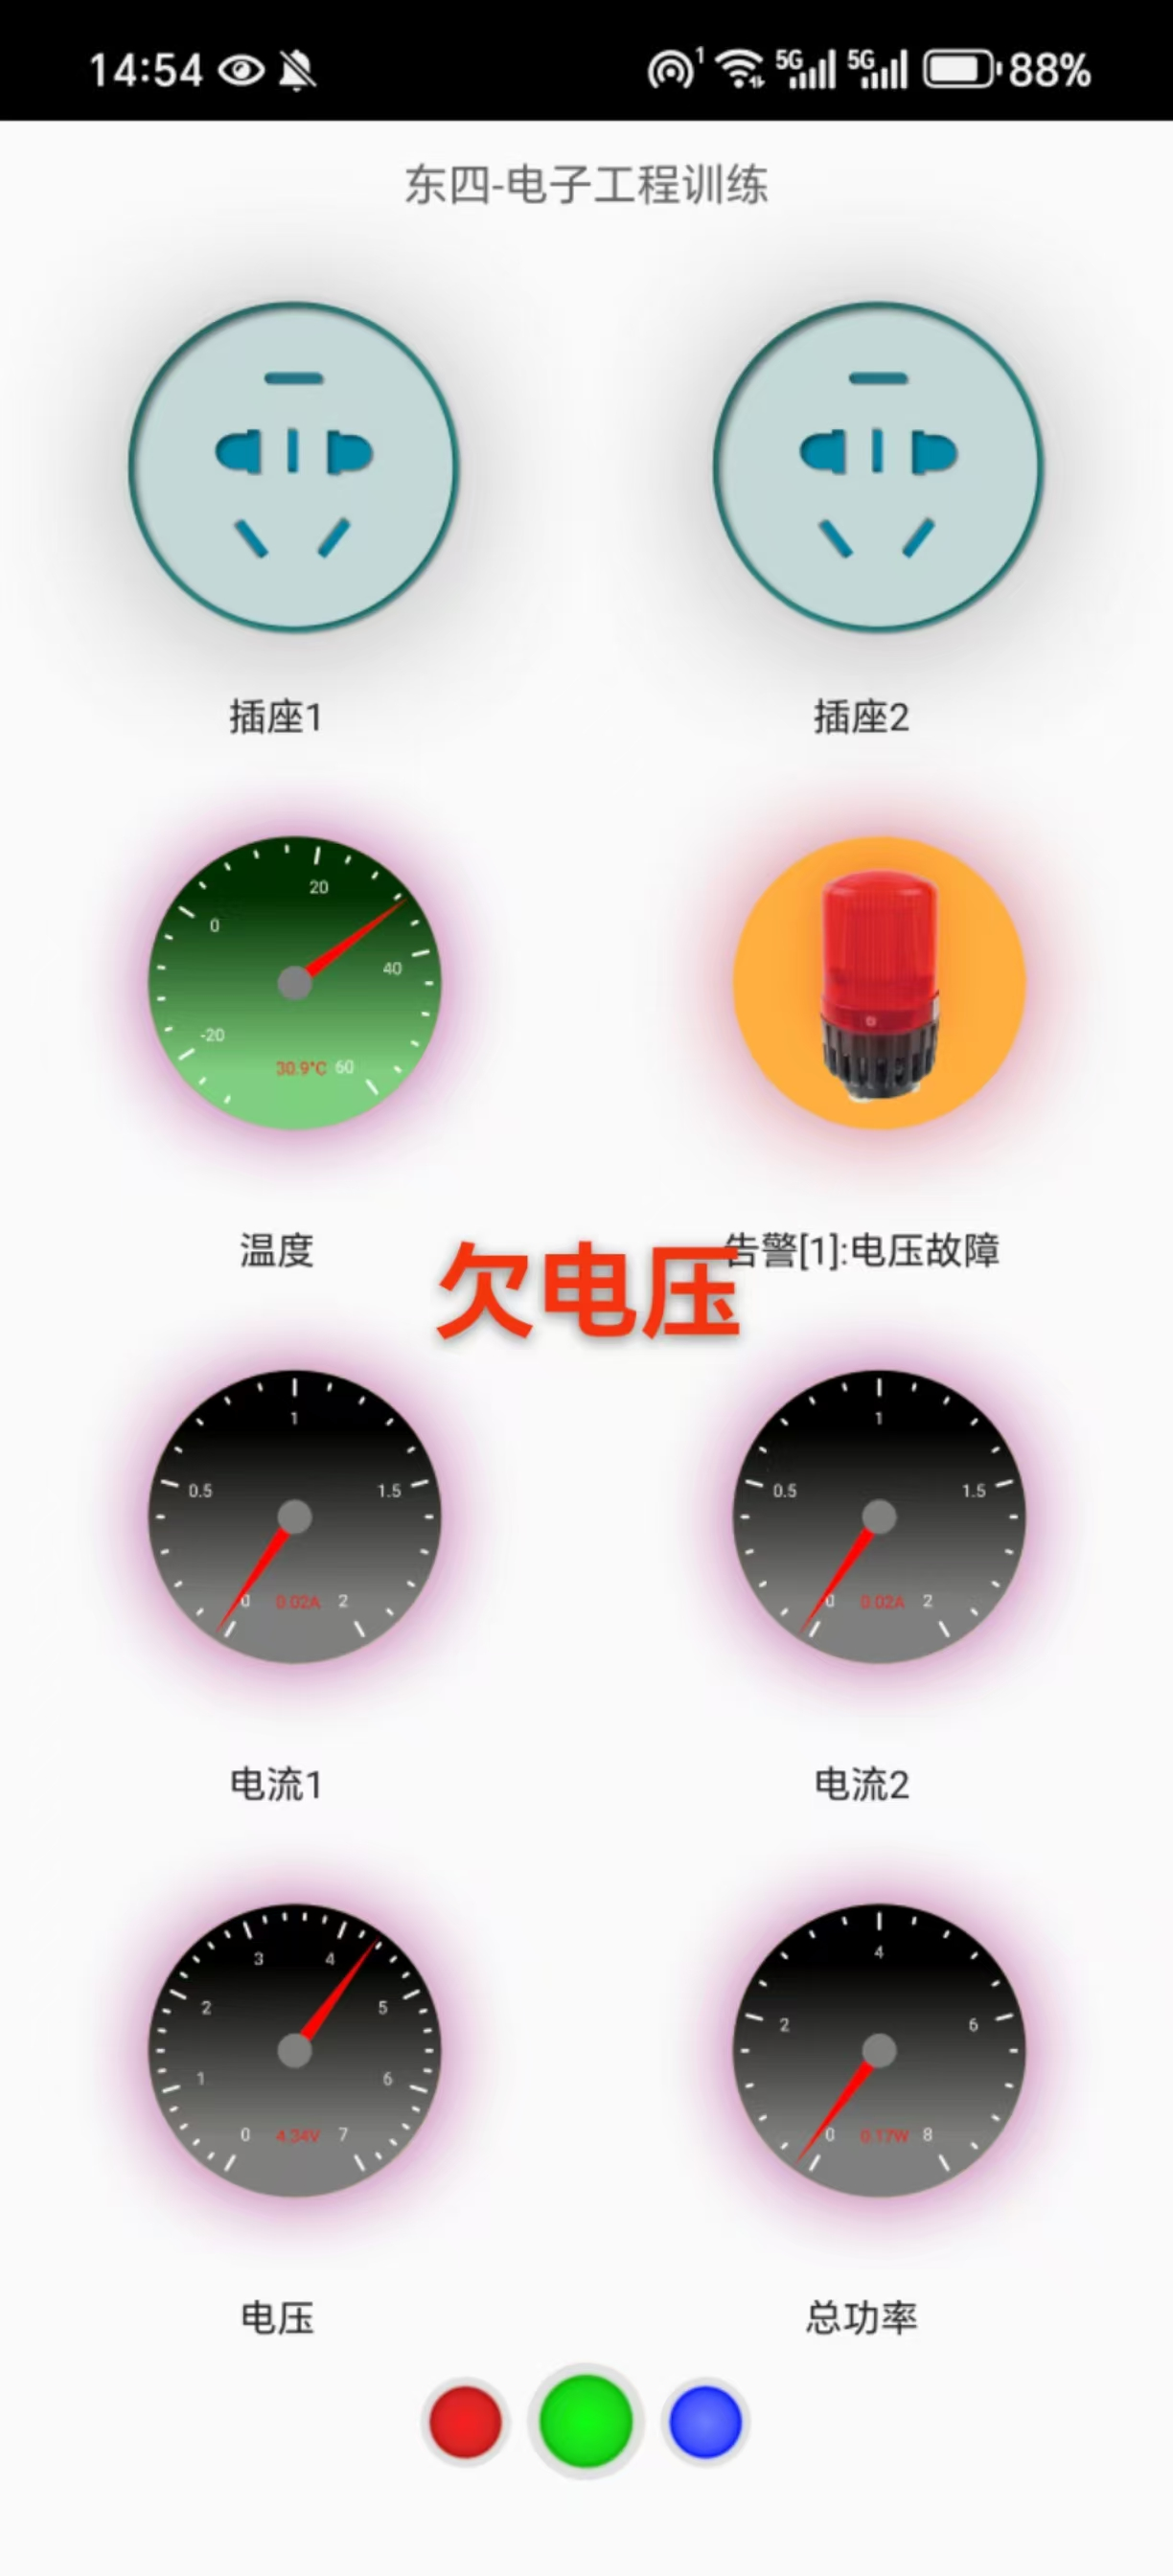
\includegraphics[width=0.9\textwidth]{figures/lv.jpg}
    \caption{欠电压}
  \end{minipage}%
  \begin{minipage}[b]{0.33\linewidth}
    \centering
    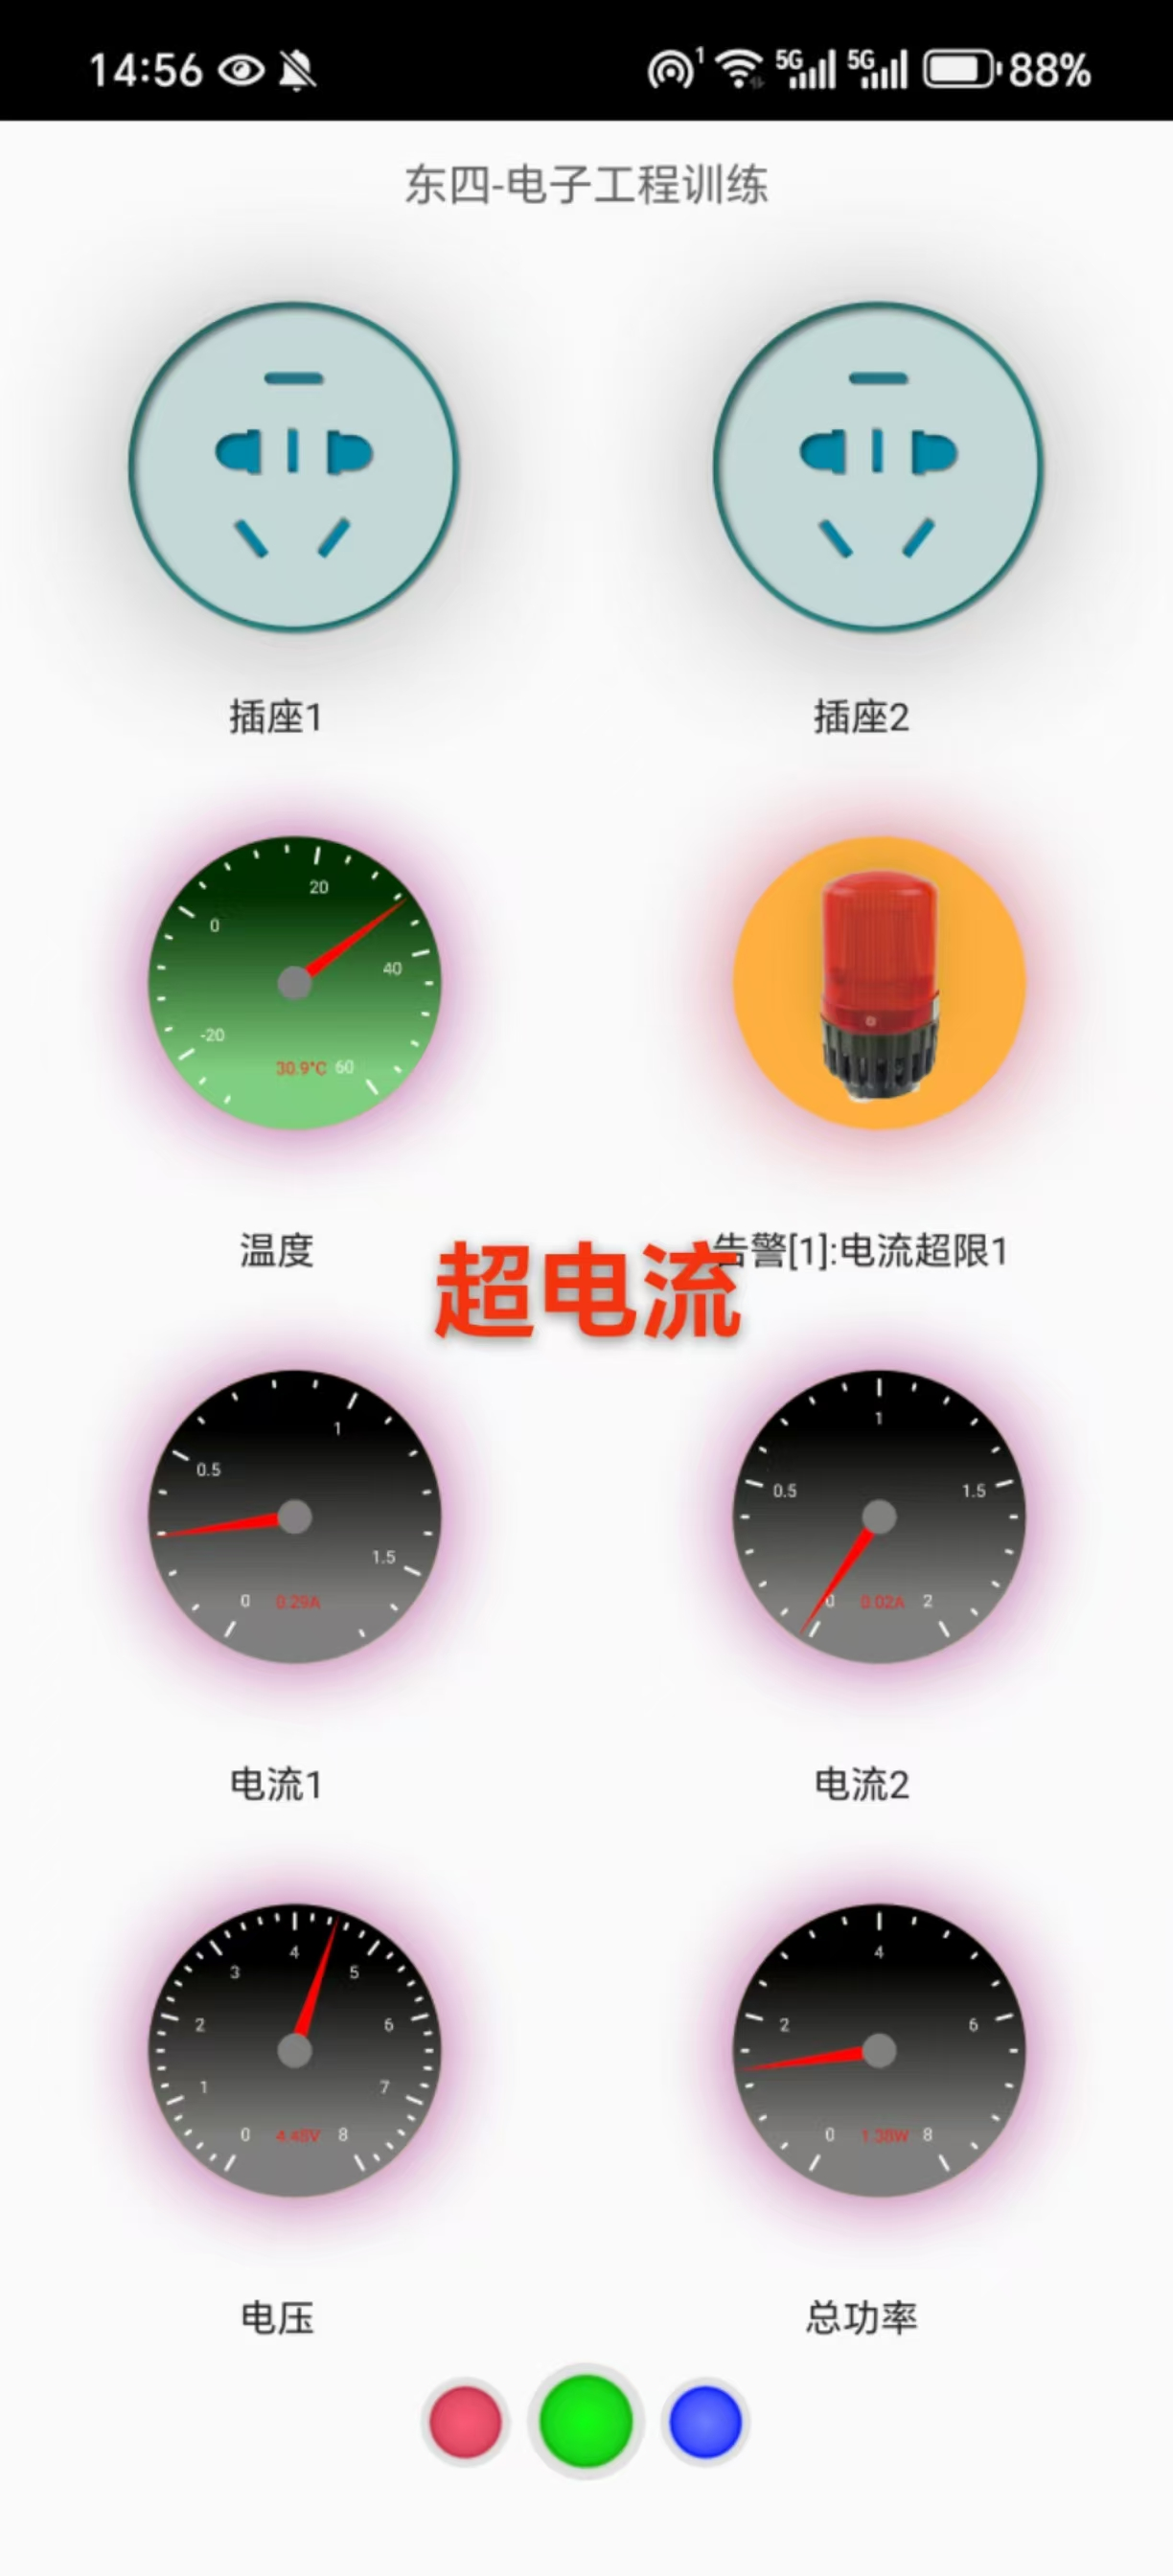
\includegraphics[width=0.9\textwidth]{figures/hi.jpg}
    \caption{超电流}
  \end{minipage}%

\end{figure}
\subsubsection{超功率}

【测试用例描述】：
\begin{enumerate}
  \item 将风扇插在插座1上，关闭插座1电源
  \item 将电流上限设定为1W
  \item 开启插座1电源，启动风扇3挡，预期超电流告警
\end{enumerate}

【测试目的】：测试插座开关超功率报警功能

【测试过程及其结果】：结果符合测试预期，
实时显示功率在超过1w时瞬间报警，
小程序显示功率超限，插座断电，
插座开关超功率报警功能良好

\subsubsection{高温}

【测试用例描述】：
\begin{enumerate}
  \item 将风扇插在插座1上，关闭插座1电源
  \item 将温度上限设定为$32^\circ C$
  \item 开启插座1电源，将手指贴在温度传感器上，预期温度超过$32^\circ C$时高温告警
\end{enumerate}

【测试目的】：测试插座开关高温报警功能

【测试过程及其结果】：结果符合测试预期，
实时显示温度在超过$32^\circ C$时瞬间报警，
小程序显示温度异常，插座断电，
插座开关高温报警功能良好

\subsubsection{低温}
\begin{enumerate}
  \item 将风扇插在插座1上，关闭插座1电源
  \item 将温度下限设定为$30^\circ C$
  \item 开启插座1电源，用小风扇吹温度传感器使之报警，预期温度低于$30^\circ C$时低温告警
\end{enumerate}

【测试目的】：测试插座开关低温报警功能

【测试过程及其结果】：结果符合测试预期，
实时显示温度在低于$30^\circ C$时瞬间报警，
小程序显示温度异常，插座断电，
插座开关低温报警功能良好

【附图】：
\begin{figure}[H]
  \centering
  \begin{minipage}[b]{0.33\linewidth}
    \centering
    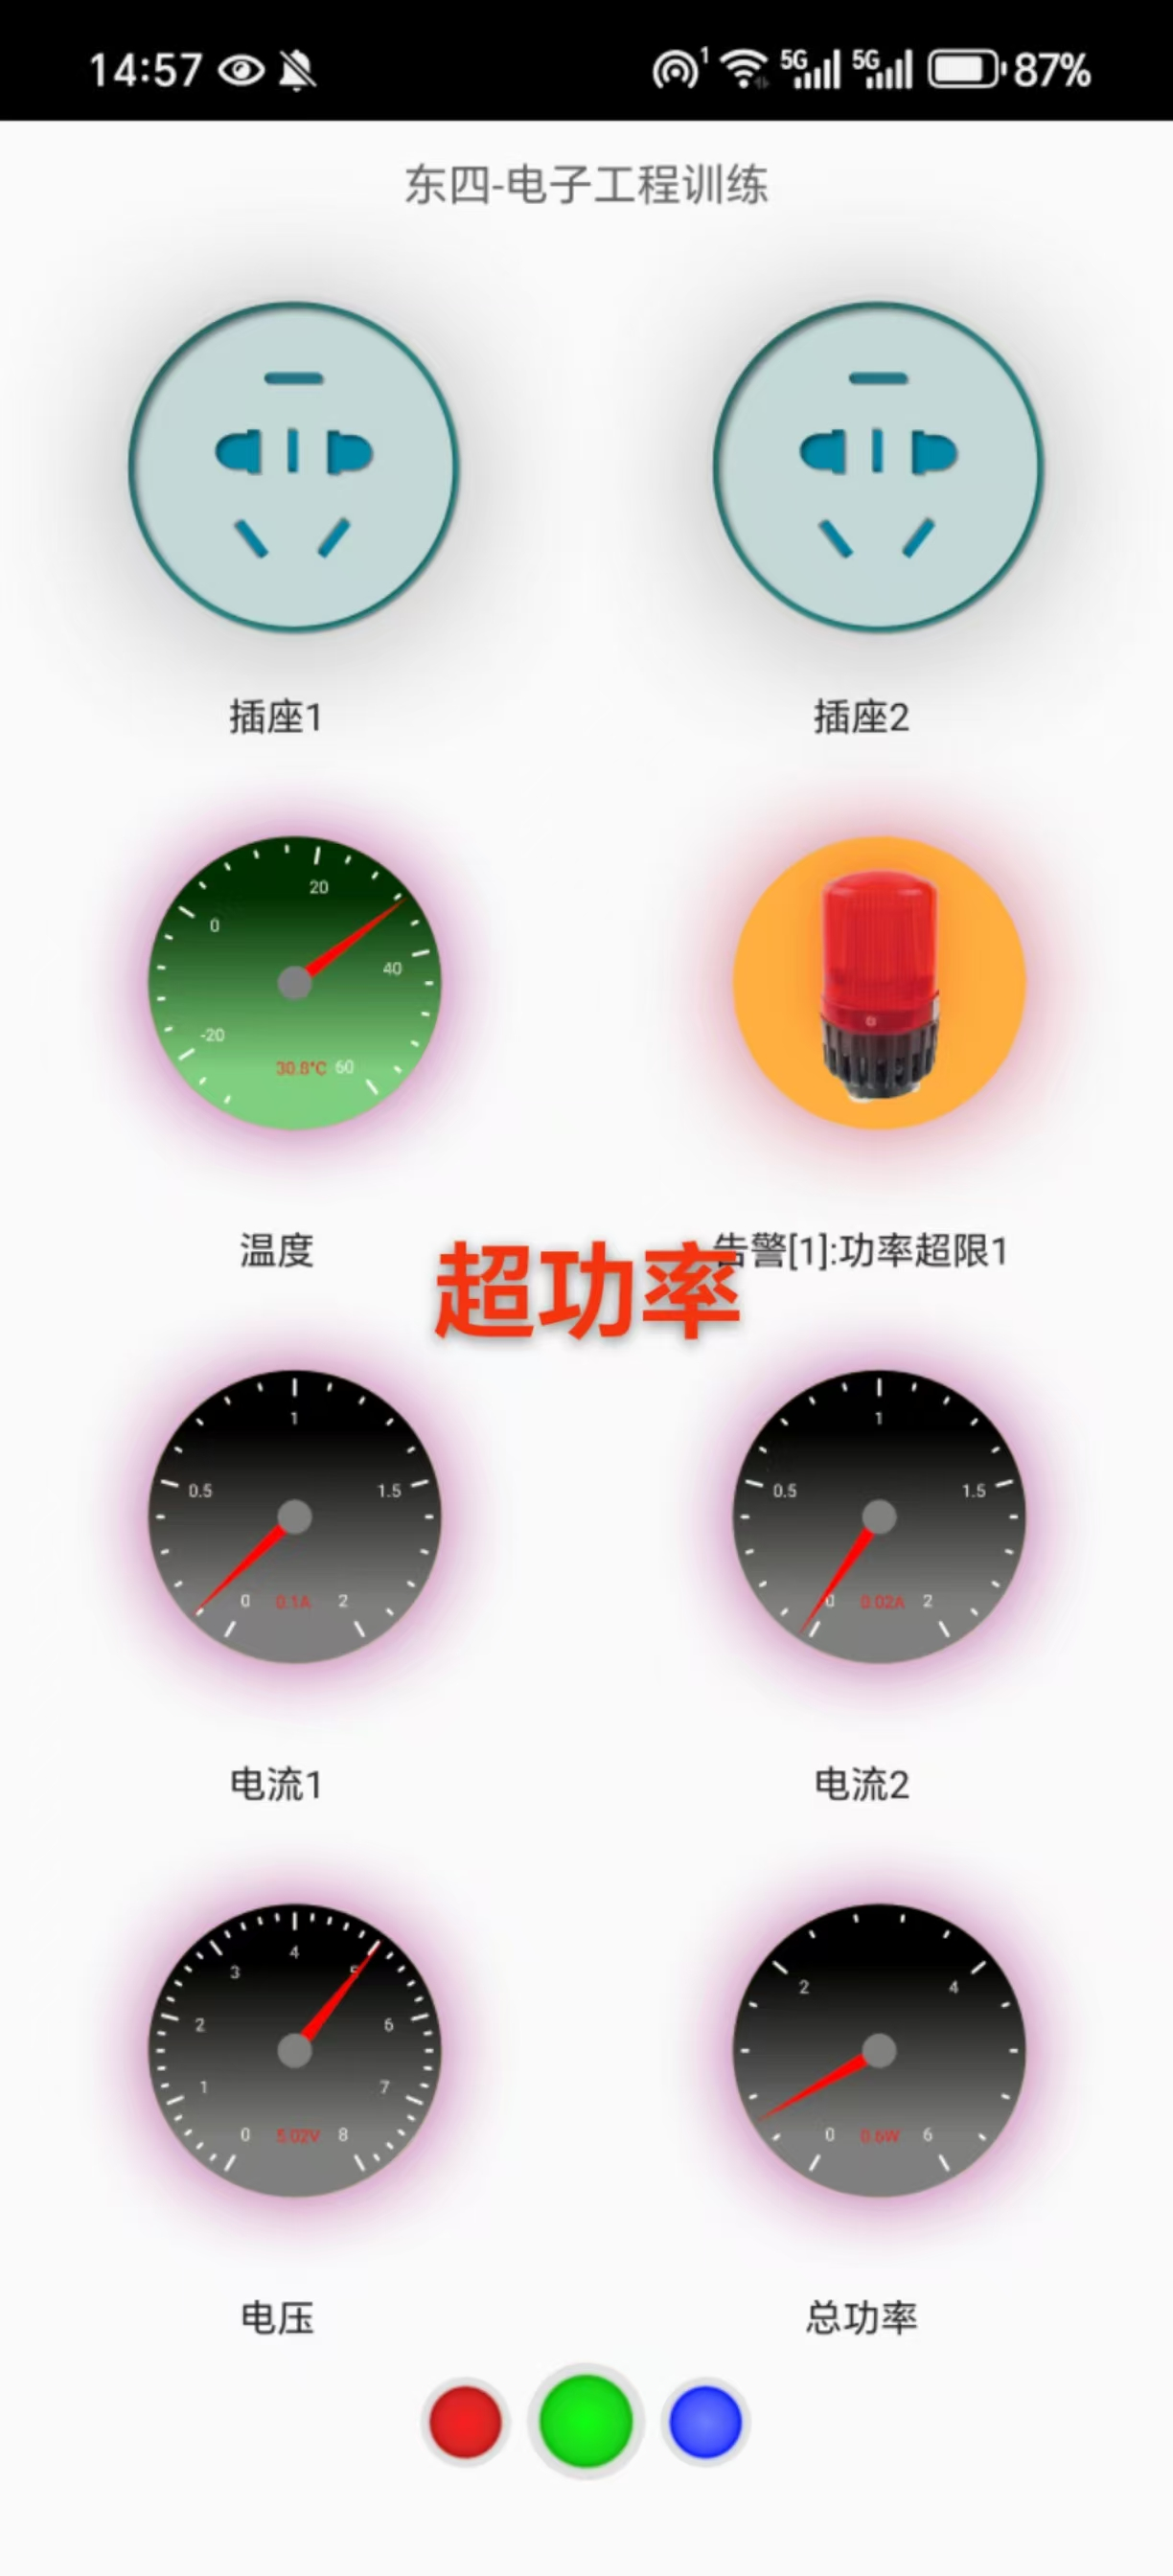
\includegraphics[width=0.9\textwidth]{figures/hp.jpg}
    \caption{超功率}
  \end{minipage}%
  \begin{minipage}[b]{0.33\linewidth}
    \centering
    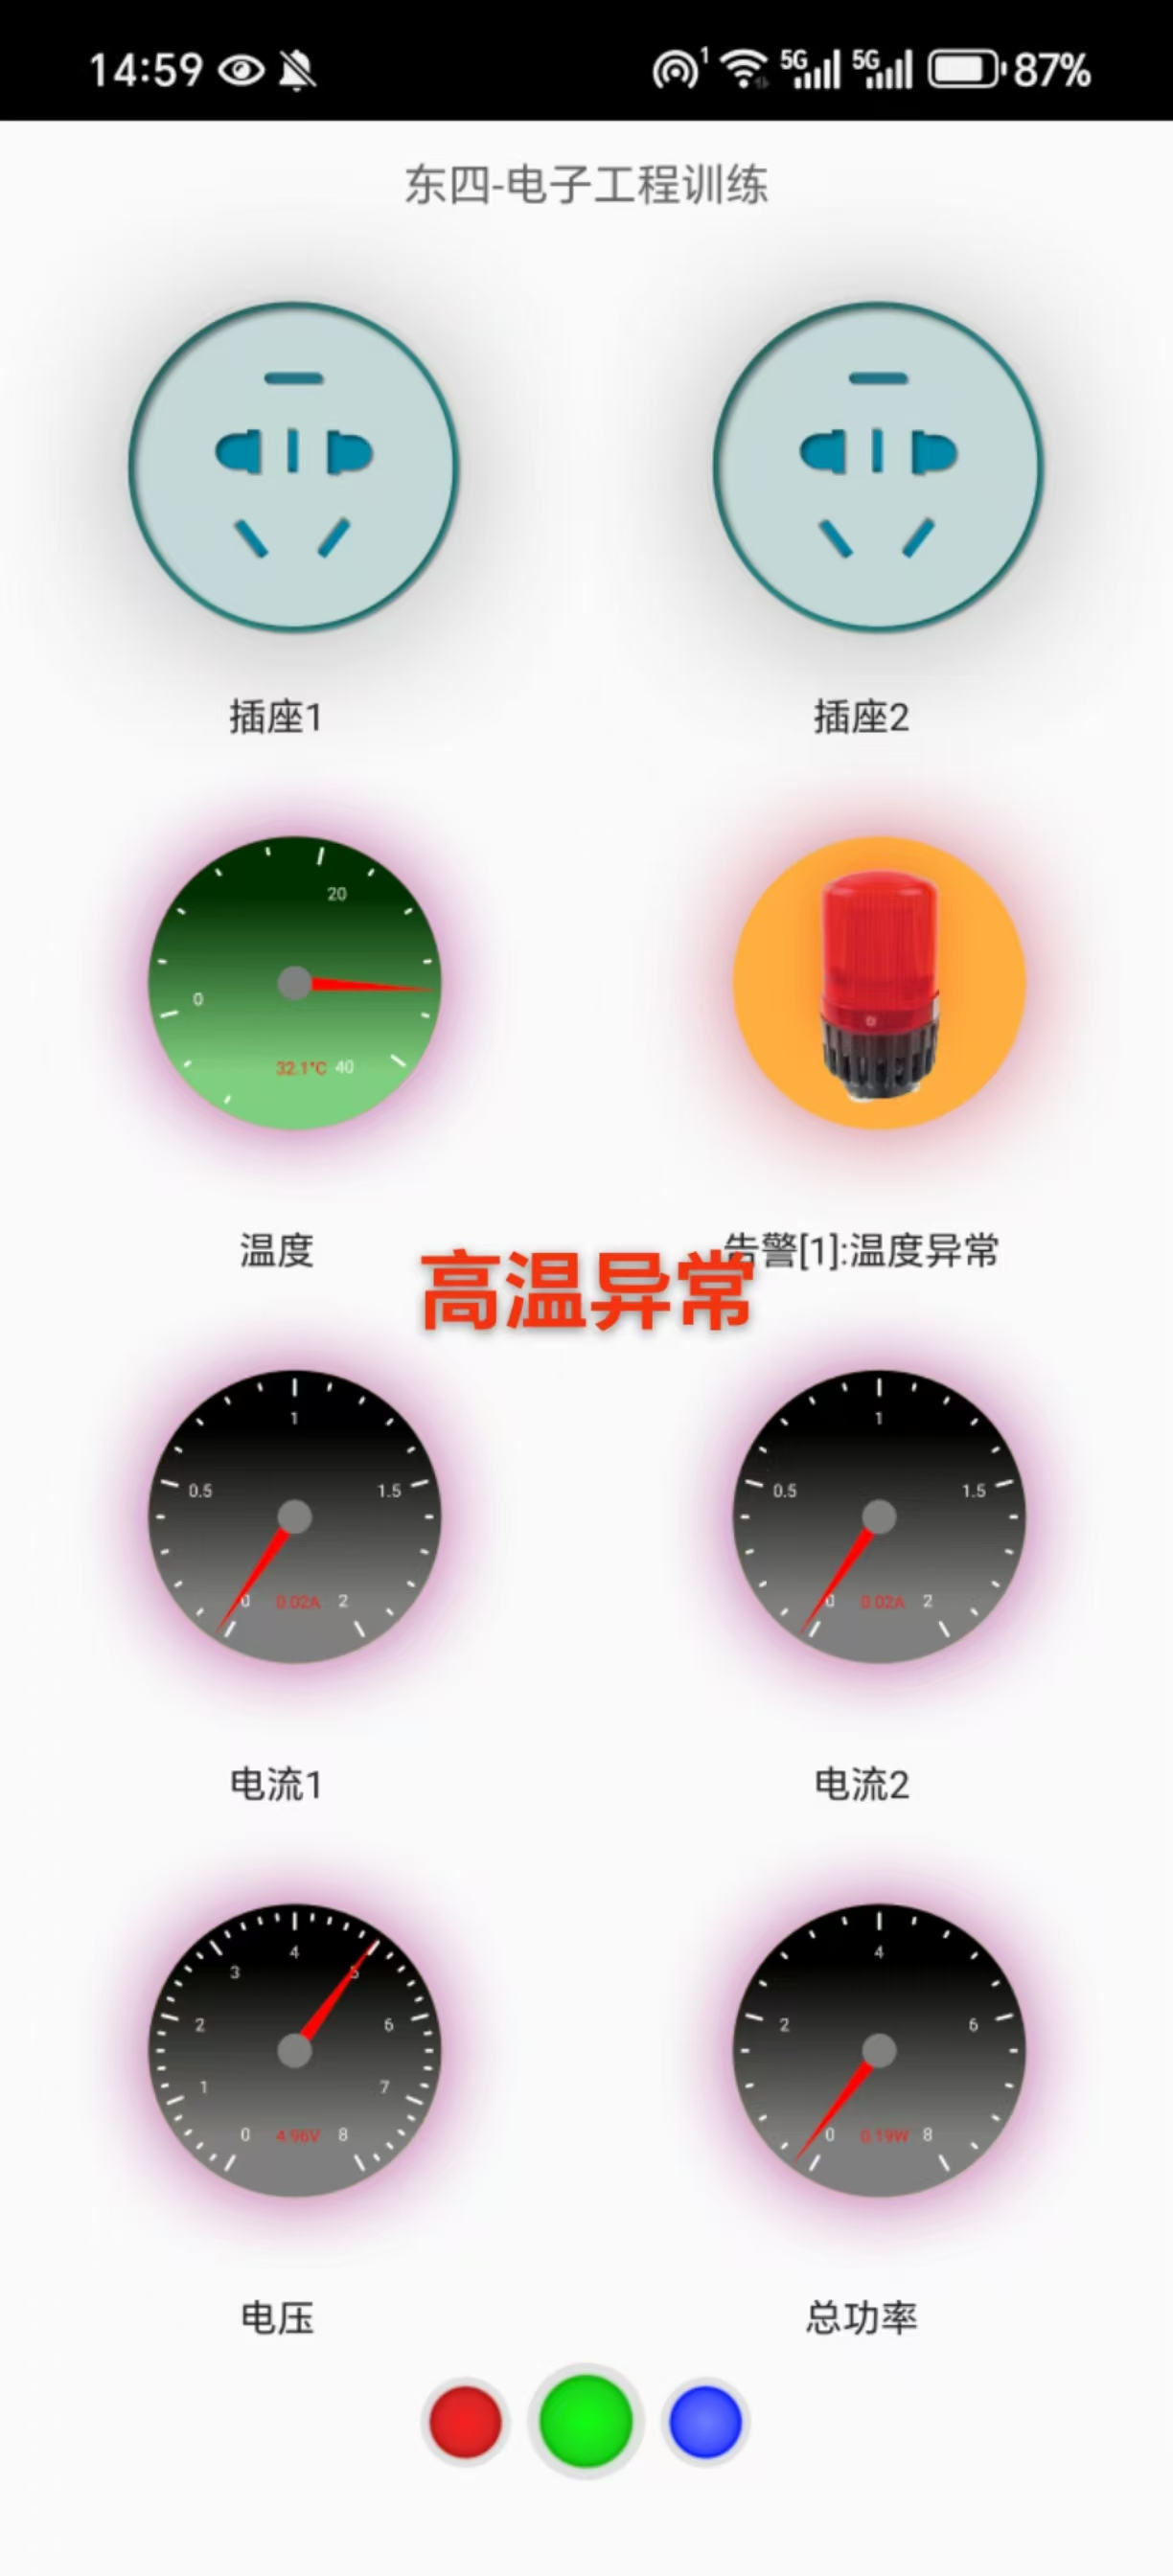
\includegraphics[width=0.9\textwidth]{figures/ht.jpg}
    \caption{高温}
  \end{minipage}%
  \begin{minipage}[b]{0.33\linewidth}
    \centering
    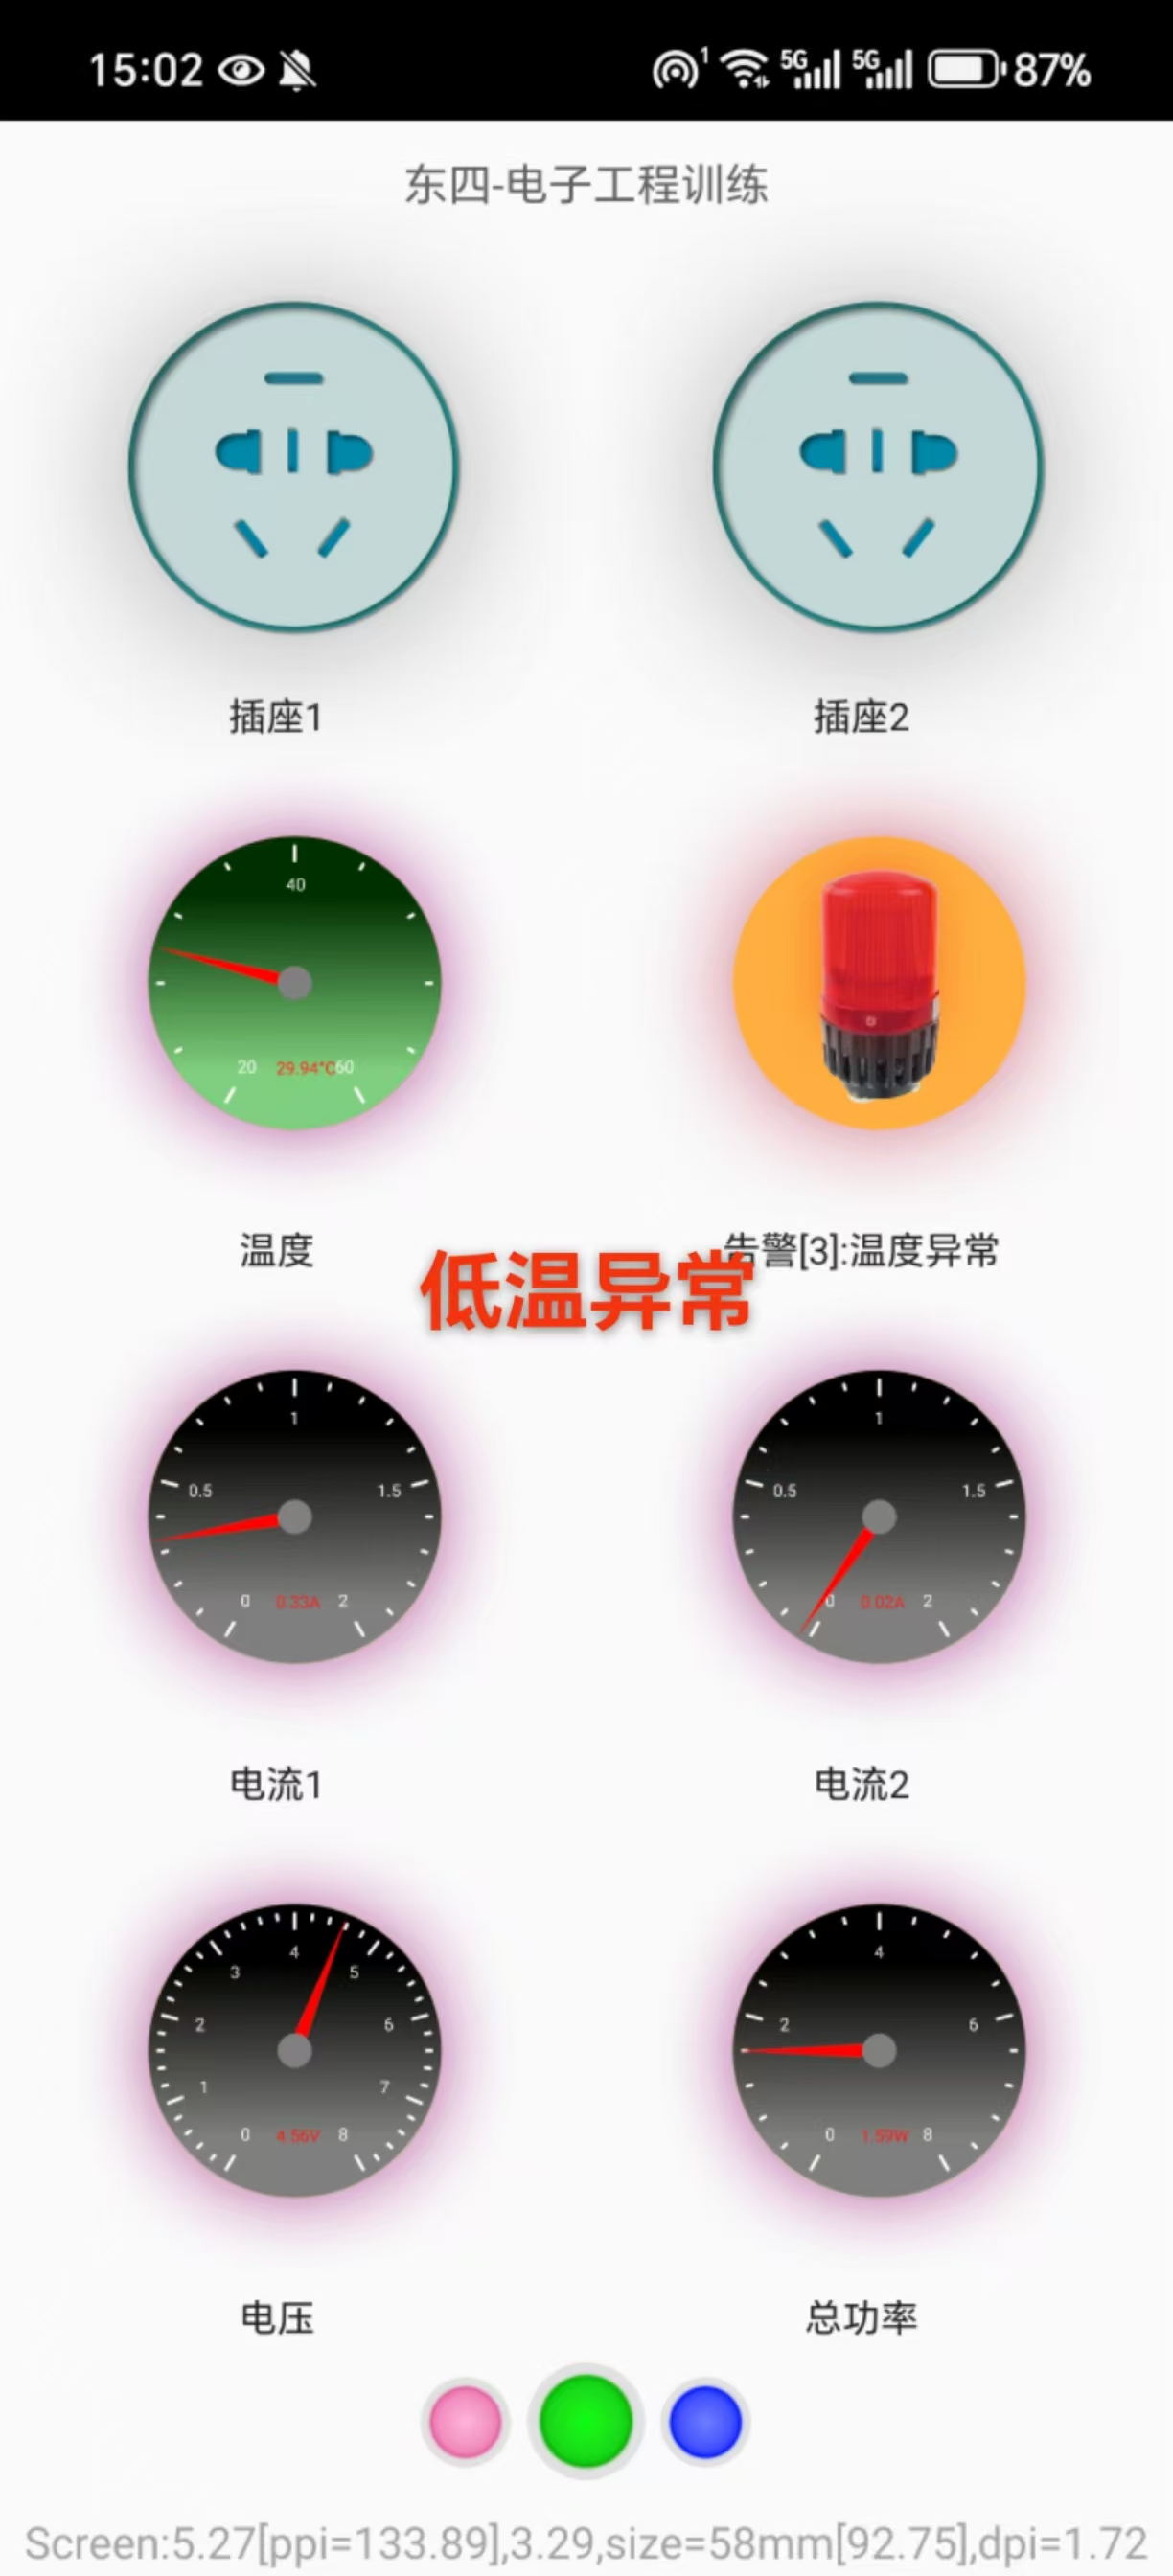
\includegraphics[width=0.9\textwidth]{figures/lt.jpg}
    \caption{低温}
  \end{minipage}%

\end{figure}

\section{实验收获与实验总结}

\subsection{实验收获}

\begin{enumerate}
\item \textbf{硬件电装与调试能力提升}
\begin{itemize}
\item 学会了如何焊接多元件的PCB板，了解了工程焊接的“焊接-调试”原则，掌握了分模块电装调试的方法
\item 学会了如何借助原理图分析电路路径，设计调试方案
\end{itemize}

\item \textbf{软硬件联调技能提高}
\begin{itemize}
\item 学会了通过Arduino IDE编写固件代码,用串口监视器进行通讯
\item 学会了软硬件参数标定方法，通过调节可变电阻拟合温度，通过计算公式拟合电流，确保传感器测量值与实际值一致
\item 学会了设计移动平均滤波器，有效抑制PWM设备电流波动（±20mA→±3mA）
\item 了解了按键的抖动原因，学会了通过写消抖函数来 减少毛刺带来的按键误识别
\end{itemize}

\item \textbf{掌握系统测试方法}
\begin{itemize}
\item 学会了系统测试方法，掌握"设计测试用例→实践验证→修正"的完整测试流程
\end{itemize}

\end{enumerate}

\subsection{实验总结}
本次实验通过自主焊接、调试、系统测试智能插座的硬件电路，并结合软件编程实现功能控制与数据采集，让我们系统性地掌握了电子产品从需求分析到原型机开发的全流程。重点实践了模块化电装与分步调试的方法、硬件参数标定技术、软硬件协同调试技巧，以及通过测试用例验证系统功能的工程思维。

实验中遇到的虚焊等问题，进一步强化了我们对细节严谨性和工程规范重要性的认识，
例如焊接顺序、元器件焊接极性等。
通过完整参与研发流程，我们对复杂工程问题的系统性解决能力得到显著提升。
\end{document}
